\documentclass[a4paper, 11pt]{tubsreprt}
\usepackage[ngerman]{babel}
\usepackage[utf8]{inputenc}
\usepackage{cite}
\usepackage{graphicx}
\usepackage{wrapfig}
\usepackage{subfigure}
\title{Wärmebehandlung}
\date{Wintersemester 17/18}
\author{J. Hansen, S. Vodde,
 J. Veer, T. Stein}

\logo{
	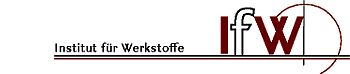
\includegraphics{Bilder/ifw-logo.jpg}
}

\begin{document}
\maketitle
\tableofcontents
\chapter{Titanwerkstoffe}

\section{Gefügemerkmale}
Wie andere Metalle liegt Titan in verschiedenen Gittermodifikationen beziehungsweise Phasenzuständen vor. Der Zustand ist von der Temperatur und den vorliegenden Legierungselementen abhängig. Bei reinem Titan liegt zwischen 1668°C und 882°C ein kubisch raumzentriertes Kristallgitter vor. Diese Phase wird als Betaphase ($\beta$-Phase) bezeichnet. Bei 882°C erfährt Titan eine Phasenumwandlung zu einem hexagonalen Gitter. Diese Phasenumwandlungstemperatur wird als Betatransus Temperatur bezeichnet und ist für jede Legierung unterschiedlich, denn die Legierungselemente haben Einfluss auf diese. \cite{Luetjering2007}.

Das hexagonale Gitter wird als Alphaphase ($\alpha$-Phase) bezeichnet. Wenn das Material langsam abgekühlt ist, liegt reines Titan bei Raumtemperatur nahezu vollständig als Alphaphase vor. 

Dieses Gitter der Alphaphase ist annähernd dichtest gepackt. Das Verhältnis in der Zelle ist etwas kleiner, als dass in der am dichtesten gepackten Zelle, c:a von $\alpha$-Titan liegt bei 1.586. Die perfekte hexagonale Zelle hat ein Verhältnis von 1.624 \cite{Siemers2017}, wobei c und a die Längen innerhalb einer Zelle sind. Je nach Aufbau der Zelle sind diese Längen unterschiedlich groß.

Die Phasenumwandlung zwischen $\beta$- und $\alpha$-Phase kann auch martensitisch erfolgen. Dabei muss das Material aus einer ausreichend hohen Temperatur abgeschreckt werden. Diese Temperatur wird als Martensitstarttemperatur bezeichnet. Sie ist wie die Betatransustemperatur von den Legierungselementen abhängig.  

\subsection{Alpha-Titan Phase}
Die alpha-Titan Phase ist durch eine hexagonale Gitterstruktur gekennzeichnet. Dadurch entsteht ein anisotropes Werkstoffverhalten in einem Korn, beziehungsweise Einkristall.
Ein Einkristall ist über ein homogenes, einheitliches Kristallgitter definiert.
In einem Belastungsfall dieses Einkristalls ist das Werkstoffverhalten abhängig von der Belastungsrichtung im Verhältnis zur Gitterrichtung. Eine Kenngröße, die das elastische Verhalten eines Werkstoffes definiert, ist das Elastizitätsmodul: 
\begin{equation}
E=\sigma*\epsilon
\end{equation}
Das Elastizitätsmodul ist das Verhältnis zwischen der anliegenden Spannung $\sigma$ und die dadurch resultierende Dehnung $\epsilon$.
Es wird in Pascal angegeben. Das Elastizitätsmodul $E$ reicht je nach Verhältnis, von minimal 100 GPa bis maximal 145 GPa. 

Jedoch wird Titan sehr selten als Einkristall hergestellt, sodass die unterschiedliche Kornorientierung dafür sorgt, dass die anisotropie der einzelnen Körner sich gegenseitig aufhebt. Somit kann man von einem isotropen Werkstoffverhalten ausgehen.


\subsection{Beta-Titan Phase}
Eine $\beta$-Phase ist ein Gefüge mit einer kubisch raumzentrierten Gitteranordnung. Dadurch resultiert ein homogenes Werkstoffverhalten.

Eine große Menge an $\beta$-Phase existiert in der Regel bei Raumtemperatur nur unter bestimmten Bedingungen. Sie kann als metastabile Phase auftreten, was bedeutet, dass das Material nicht vollständig den Phasenübergang abschließen konnte und so in dem Zustand aus höheren Temperaturen verblieben, "eingefroren" ist.  

Durch Zusatz bestimmter Legierungselemente kann die $\beta$-Phase auch in größeren Mengen vorliegen. Dies wird im Kapitel "betastabilisierende Legierungselemente" näher erläutert.
\subsection{Gefüge}
Ausgehend von grundlegend verschiedenen Gefügen können diese durch Wärmebehandlung hinsichtlich ihrer mechanischen Eingenschaften optimiert werden. Eine Kombination aus mehreren Gefügeausprägungen können die Vorteile der einzelnen kombinieren. Dazu werden mehrstufige Wärmebehandlungen eingesetzt. Die Proben, die verwendet werden, können nicht mehr Rekristallisiert werden, sodass die verbleibenden Wärmebehandlungen auf Parameter wie Korngröße kaum Einfluss nehmen können. Das Gefüge ist somit von dem Ausgangsgefüge abhängig.  
\subsubsection{Lamellar}
Lamellare Gefüge sind unabhängig von dem Ausgangsgefüge einstellbar. Sie entstehen aus einer Abkühlung aus dem $\beta$-Gebiet. Während des Abkühlens bilden sich in den Korngrenzen der $\beta$-Phase $\alpha$-Bereiche, die in das $\beta$-Korn hinein wachsen. Die Alphabereiche wachsen erst in eine Richtung bevor sie ihre Dicke erhöhen. Je nach Abkühlgeschwindigkeit entstehen so dünne oder dickere Nadeln. Die Abbildung 1.1 zeigt ein beispielhaftes Gefüge, indem voll lamellare Strukturen zu sehen sind. Lamellare Gefüge werden auch als Widmannstättengefüge bezeichnet \cite{Luetjering2007}.


\begin{figure}


	\centering
		\includegraphics[scale=1]{Bilder/lamellar.jpg}
		\captionof{figure}[lamellares Gefüge]{Volllamellares Gefüge \cite{Leyens2002}}
		\label{lamellar}
		
\end{figure}
\subsubsection{Martensit}
Der Martensit ist eine spezielle Form unter den Gefügen, da dieser der einzige ist in denen die Phasen metastabil vorliegen. Er resultiert aus einer schnellen Abkühlung bei Temperaturen höher als als die Martensitstarttemperatur. Bei diesen Temperaturen ist das Volumenverhältnis zwischen $\alpha$ und $\beta$ in dem diese stabil vorliegen ein anderes, als das bei niedrigen Temperaturen. Bei einer langsamen Abkühlung würde sich die Betaphase in Alphaphase umwandeln. Aufgrund der schnellen Abkühlgeschwindigkeit von über 1000°C/min können diese Diffusionsvorgänge nicht abgeschlossen werden. Somit kommt es zu einem diffuisonslosen Phaseübergang \cite{Luetjering2007}. Aufgrund der unterschiedlichen Gitterstruktur von Alpha und Beta, kommt es zu dem charakteristischen Martensitgefüge wie in Abbildung \ref{vollmartensit} zu sehen ist.

\begin{figure}
\centering
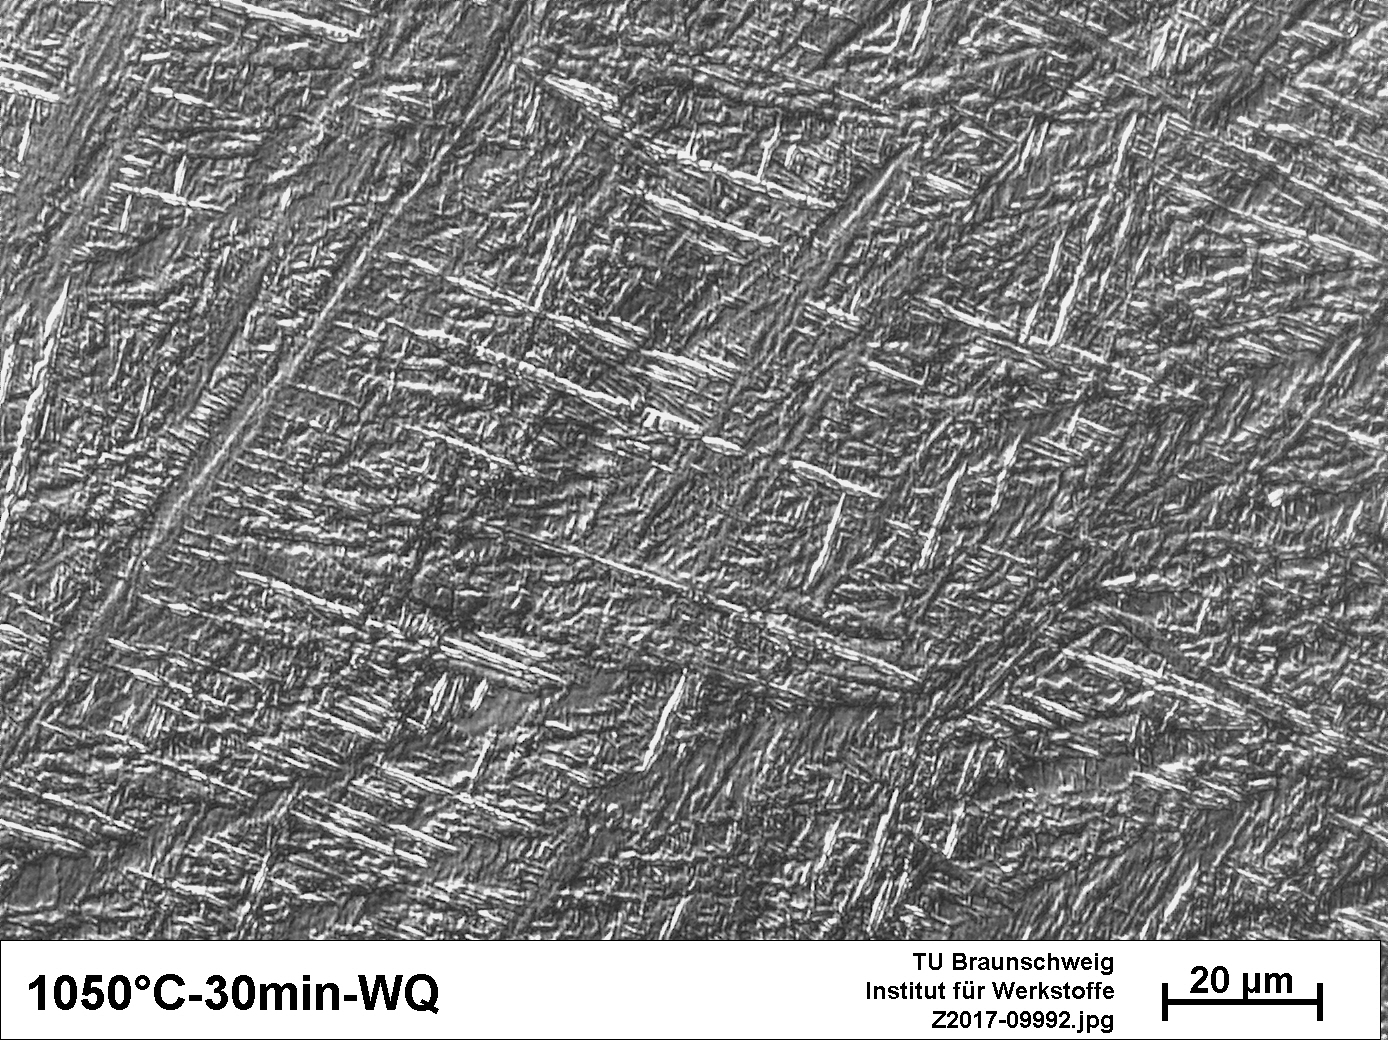
\includegraphics[scale=0.5]{Bilder/Vollmartensit.jpg}
\caption{Vollmartensitisches Gefüge}
\label{vollmartensit}
\end{figure}
\subsubsection{Globular}
Globulare Phase besteht aus großen, runden $\alpha$-Bereichen. Dieses Gefüge ist charakteristisch für eine Probe, welche noch keine Wärmebehandlung erfahren hat. Es lassen sich hieraus viele andere Gefüge einstellen. In Abbildung \ref{globular} erkennt man ein solches Gefüge. 
\begin{figure}
\centering
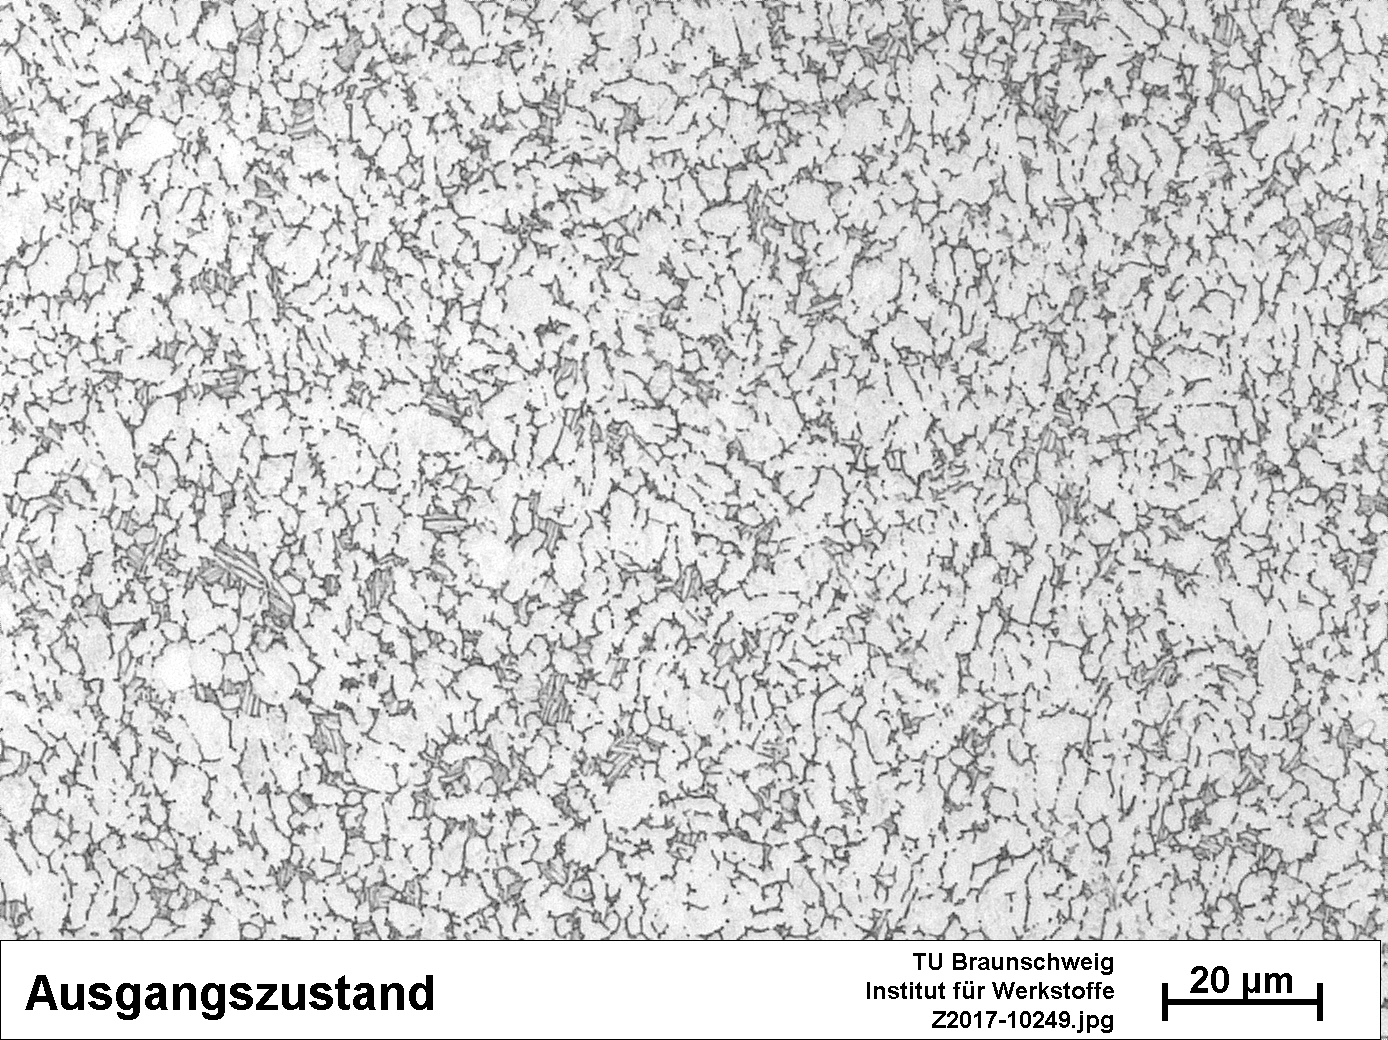
\includegraphics[scale=0.6]{Bilder/Ausgangsgefuege.jpg}
\caption{Globulares Gefüge}
\label{globular}
\end{figure}

\subsubsection{Bi-Modal}
Bi-Modal-Gefüge(Duplex-Gefüge) sind durch globularer $\alpha$-Phase und Lamellen aus $\alpha$- und $\beta$-Phase gekennzeichnet. Das Gefüge kombiniert rein globulare Alphaphase mit lamellaren Anteilen. In Abbildung \ref{bimodal} ist ein solches Gefüge zu erkennen. 
\begin{figure}
\centering
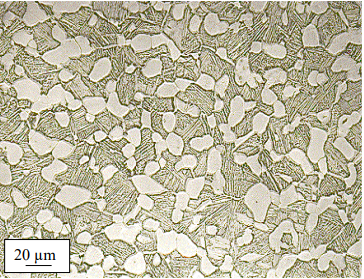
\includegraphics[scale=1]{Bilder/Duplexgefuege.PNG}
\caption[Bi-Modal-Gefüge]{Bi-Modal-Gefüge\cite{Werkstoffdesign2012}}
\label{bimodal}
\end{figure}

\chapter{Methodik}
\section{Intermetallische Verbindung}
Titanlegierungen können, wie alle anderen Metalllegierungen, intermetallische Verbindungen bzw. Phasen bilden. Der Gittertyp der Phase passt meist nicht zu den Gittertypen der einzelnen Komponenten [vgl. Domke (1986)]. Abhängig vom Gittertyp der Grundmatrix und der Verbindung,  können kohärente, teilkohärente oder inkohärente Verbindungen entstehen. Die Grenzflächenenergie der kohärenten Teilchen ist gering. Sie verzerren das Kristallgitter nur etwas. Wachsen diese zu inkohärenten Teilchen heran, steigt die Grenzflächenenergie und das Kristallgitter wird stärker verzerrt.

Bestimmte Titanlegierungen nutzen diese intermetallischen Phasen, um die mechanischen Eigenschaften auch bei höheren Temperaturen zu Verbessern \cite{Luetjering2007}.

Reines Titan kann keine intermetallischen Phasen bilden. Ausschlaggebend hierfür sind die Legierungselemete, die $\alpha$- und $\beta$- Stabilisatoren.  Diese Phasen lassen sich wie die Stabilisatoren  in $\alpha$- und $\beta$- Phasen aufteilen.  
\subsection{$\alpha$-Phasen}
Mit steigendem Aluminium Äquivalent können sich intermetallische Titan-Aluminium-Phasen bilden, die bei Raumtemperatur beständig sind. Wie das Diagramm ……….. zeigt, beginnt dieser Vorgang bereits bei ca. 5 \% Aluminium. Das zwei Phasen Gebiet $alpha$Ti und Ti3Al bildet sich. Für die meisten Titanlegierungen gilt jedoch der Richtwert von 6 \% Aluminium um Ti3Al ($\alpha2$) Teilchen auszuscheiden.  Die Ti3Al Teilchen besitzen eine hexagonale Gitterstruktur wie das $\alpha$Ti. Die Teilchen können  die gleichen Gitterplätze besetzten und verzerren das Kristallgitter nur wenig. Sie sind kohärent.
Werden noch größere Anteile Aluminium  zum Titan legiert, kann sich TIAl ( $\gamma$-TiAl) bilden. Diese Teilchen besitzen ein Tetragonales Kristallgitter.
 Werden Legierungen mit diesen beiden genannten Phasen erzeugt, entstehen sogenannte Titan-Aluminide \cite[vgl.]{Luetjering2007}.   

\subsection{$\beta$-Phasen}
Intermetallische $\beta$-Phasen sind in Titanlegierungen unerwünscht, da sie die mechanischen Eigenschaften verschlechtern. Die isomorphen Stabilisatoren, wie Molybdän, Vanadium oder Niob, bilden in gewöhnlichen Legierungen keine intermetallischen Phasen. Ihre Legierungsanteile sind zu gering. Die eutektoiden Stabilisatoren, wie Chrom oder Eisen hingegen, bilden diese. TiFe und Ti2Cr Phasen sollen in Titanlegierungen nicht entstehen \cite{Luetjering2007}.

\section{Rasterelektronenmikroskopie}
Das Rasterelektronenmikroskop (REM) bietet eine bessere Auflösung und eine größere Vergrößerung, als das Auflichtmikroskop. Es können Vergrößerungen von bis 100000 x erreicht werden. Die Auflösung liegt bei wenigen Nanometer. Durch eingebaute Detektoren am REM können bestimmte analytische Methoden zusätzlich  durchgeführt werden. Dies ist hilfreich für Auswertung der Proben.
Eine Wolframdraht oder ein Lanthanhexaborideinkristall ($LaB_{6}$) dient als Elektronenquelle. Die Elektronen werden emittiert und mittels Beschleunigungsspannung in Richtung Anode abgelenkt. Je nach Auflösung kann die Spannung zwischen 200$V$ und 50$kV$ liegen. Elektromagnetische Linsen bündeln die Elektronen in einem Strahl und lenken ihn auf die Probe. Mit einer Anblenkspule kann der Strahl über die Probe geführt werden \ref{REM Bild}.

\begin{figure} %REM Aufbau
\centering
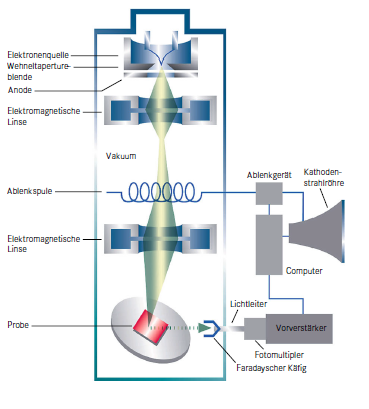
\includegraphics[width=0.5\textwidth]{Bilder/REM.png}
\caption{Aufbau eines Rasterelektronenmikroskops}
\label{REM Bild}
\end{figure}

Die Elektronen gelangen auf die Probeoberfläche und es entstehen Wechselwirkungen zwischen den Strahlelektronen und den Atomen der Probenoberfläche. Die zwei wichtigsten Erscheinungen sind hierbei die Rückstreuelektronen (RE) und die Sekundärelektronen (SE). Die Strahlelektronen werden durch die Atomkerne in der Probe abgelenkt  und verlieren an Energie. Diese Energie wird in Form der Röntgenbremsstrahlung frei. Die dabei teilweise zurückgeworfenen Elektronen werden als RE bezeichnet. Der Streuprozess zwischen den Strahlelektronen und den Elektronen in den Atomschalen, führt zu SE. Die hierbei entstehende Röntgenstrahlung, ist die charakteristische Röntgenstrahlung. Die Elektronen in den Atomschalen werden von den Strahlelektronen herausgeworfen. Die Schale ist ionisiert. Diese freien Plätze werden durch andere Elektronen besetzt. Die dabei freiwerdende Energie wird in Form von Röntgenstrahlung emittiert. Verlassen RE die Probe können zusätzlich SE entstehen.
Die SE und RE dienen nun der Bilderzeugung. Die Elektronen werden mit jeweils unterschiedlichen Detektoren erfasst. Die Spannung, die aus dem Detektorimpuls erzeugt wird, gelangt zur Kathodenstrahlröhre. Werden viele Elektronen erfasst, steigt die Spannung und der Bildpunkt erscheint hell. Die einzelnen Bildpunkte werden nun durch das „abrastern“ der Oberfläche erzeugt. Heutzutage erfolgt die Bildherstellung digital. [vgl. Romeis Mikroskopische Technik (2015)].
Gute Bildergebnisse können nur durch eine sorgfältige Probepräparation entstehen. Die Oberflächen müssen sauber sein. Die Proben sollten vor der Analyse im Ultraschallbad gereinigt werden.  Zudem muss die gesamte Probe elektrisch leiten. Eingebettete Proben können nicht verwendet werden. Der Kunststoff nimmt die Elektronen auf und würde den Elektronenstrahl ablenken. Als alternative kann eine leitende Gold oder Silberschicht aufgebracht werden.
\section{Wärmebehandlung}

Die Wärmebehandlung nach der Rekristllisation ist die letzte Methode um das Gefüge des Titans einzustellen. Hierbei kommt es auf Parameter wie Temperatur, Haltezeit und Abkühlmethode an. Um die bereits erwähnten Gefüge zu realisieren, ist eine spezifische Abfolge von einer beziehungsweise mehreren Stufen einer Wärmebehandlung nötig. Die grundlegenden Behandlungen werden in diesem Kapitel behandelt, wobei die speziellen, mehrstufigen Behandlungen im dritten Kapitel behandelt werden.
\paragraph{Temperaturkontrolle}
Für die Temperaturkontrolle innerhalb der Wärmebehandlung kommt ein Ofen zum Einsatz. Dieser kann bis Temperaturen deutlich oberhalb der Betatransustemperatur aufheizen und diese, mit einer Genauigkeit von drei Kelvin, halten. So kann der Temperaturbereich, der für die Wärmebehandlungen wichtig ist, eingestellt werden. Dieser liegt zwischen Raumtemperatur und 50°C - 100°C oberhalb der Betatransustemperatur vor. Der Ofen ist außerdem für die Aufheizgeschwindigkeit verantwortlich, da diese auch einen wichtigen Einfluss haben kann.

\paragraph{Abkühlmedien}

Durch Abkühlmedien werden bestimmte Abkühlgeschwindigkeiten realisiert. Für langsamere Abkühlungen als in der Luft wird der Ofen genutzt. Hier kann die Temperatur beliebig langsam reduziert werden. Ein weiterer Vorteil des Ofens ist, dass die Probe auf eine bestimmte Temperatur herunter gekühlt werden kann. Dies ist für mehrstufige Wärmebehandlungen wichtig, bei denen eine Abkühlung auf Raumtemperatur zwischen den Schritten vermieden werden soll. 

Da der Ofen nicht überaus schnell abkühlen kann, wird zur schnelleren Abkühlung Luft mit Raumtempertur verwendet. Durch den höheren Temperaturgradienten im Verhältnis zum Ofen wird so die Abkühlung beschleunigt.  

Um noch schnellere Abkühlungen zu realisieren wird Wasser oder Öl verwendet. So werden zum Beispiel Abkühlgeschwindigkeiten für eine Martensitbildung ermöglicht. Die hohe Abkühlgeschwindkeit von gewöhnlich mehr als 1000$K$/min verhindert das element partitioning. So können sich neben dem Martensit, Alpha-Beta-Verhältnisse einstellen, die bei langsamen Abkühlungen nicht möglich sind. 
\subsection{Anpassung der Gefüge durch Wärmebehandlung}
\begin{figure}
	\centering
	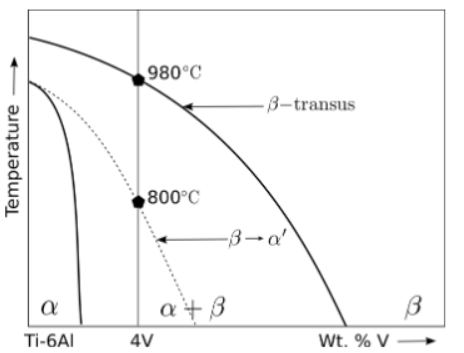
\includegraphics[scale=0.9]{Bilder/Phasendiagram.PNG}
	\caption[Phasendiagramm]{schematisches Phasendiagramm Ti-6Al-4V \cite{Babu2008}}
	\label{Phasendiagram}
\end{figure}
Das Anpassen der Gefüge ist das Ziel der Wärmebehandlungen. So werden Werkstoffeigenschaften gezielt für den jeweiligen Anwendungsfall optimiert, denn bestimmte Gefüge, mit bestimmten Mechanische Eigenschaften,  folgen aus bestimmten Wärmebehandlungen. Diese Einstellung durch Wärmehandlungen hat bestimmte Grenzen. Korngröße und die daraus folgenden Eigenschaften sind nicht mehr reduzierbar. Eine Behandlung die Kornwachstum beinhaltet sollte somit mit bedacht Gewählt werden,da gewöhnlich die Festigkeit durch Kornwachstum abnimmt.
\subsubsection{Lamellar}
Rein lamellare Strukturen folgen aus einer Abkühlung aus dem $\beta$-Gebiet. In dem Phasendiagramm aus Abbildung 1.5 ist erkennbar, dass oberhalb der Betatransuslinie das Material in einem Einphasenfeld liegt und somit bei einer moderaten Abkühlung vollständig in lamellare Phase umwandelt. Wird die Glühungstemperatur unterhalb der Betatransustemperatur gewählt, ist das Material in einem Zweiphasengebiet. So können unterschiedliche Alphagehälter eingestellt werden, sodass eine Kombination aus $\alpha$-Phase und $\alpha + \beta$-Phase entsteht. Das so eingestellte $\alpha$-Gefüge wird auch als Primäralpha bezeichnet. 


Je nach Feinheit der Platten hat das Gefüge positive oder negative Eigenschaften bezüglich der Festigkeit. Fein lamellare Platten sorgen für eine zunahme der Festigkeit und grobe Platten für eine Abnahme. Dies ist durch die unterschiedliche Grenzflächendichte zu erklären, denn die hohe Anzahl an Körnern behindert den Versetzungsfortschritt. Bei großen lamellaren Platten ist es für die Versetzung deutlich einfacher durch das Bauteil fortzuschreiten. 

\subsubsection{Martensit}
Martensit entsteht mit Abkühlgeschwindigkeiten aus Temperaturen höher als die Martensitstarttemperatur. Wie bei lamellaren Gefügen kann auch eine Kombination aus Primärem Alpha und Martensit erfolgen, indem die Glühungstemperatur im 2-Phasengebiet gewählt wird. Wie hoch die Temperatur gewählt wird entscheidet über den Primäralphagehalt. 

Die charakteristische Struktur des Martesits sorgt für ein sehr festes Werkstoffverhalten. Aufgrund der kaum zu erkennenden Grenzen zwischen den Phasen, ist die Grenzflächendichte sehr hoch. Somit steigt die Festigkeit.


\subsubsection{Bi-Modal}
Diese Strukturen bestehen aus einer Kombination von primär Alpha und lamellaren Strukturen in den Betakörnern. Dies Lässt sich durch eine Wärmebehandlung einstellen in der die Glühungstemperatur unterhalb der Betatransustemperatur liegt. Die Temperatur entscheidet über die Ausprägung der primären Alphakörner. Aus dem Phasendiagramm aus Abbildung 1.5 erklärt sich, dass je höher die Glühungstemperatur ist desto geringer ist der Alphagehalt in dem resultierenden Gefüge. Die Abkühlgeschwindigkeit entscheidet über die breite der wären des Abkühlvorgangs entstehenden Lamellen \cite{Luetjering2007}.

\subsubsection{Globular}
Globulare Gefüge lassen sich auf mehrere Wege erzeugen. Zum Einen kann die Abkühlung von der Glühtemperatur so gering gewählt werden, dass die entstehenden Lamellen sehr groß werden. So entstehen Alphagehalten von 80 Volumenprozent und mehr. Zum Anderen kann die Glühungstemperatur sehr gering gewählt werden, sodass sich ein sehr hoher Alphaanteil einstellt. Dabei sollten beachtet werden, dass die Diffusionsgeschwindigkeit bei geringen Temperaturen sehr gering ist und so eine lange Haltezeit vorgesehen sein sollte. 

\section{Auswertung der Proben}
\subsection{Auszählverfahren}
Das Auszählverfahren ist ein manuelles Hilfsmittel um die Phasenanteile von Gefügen zu ermitteln. Metalllegierungen, wie auch Titan, können unterschiedliche Gefüge mit mehreren Phasen ausbilden. Deren Anteile können mit diesem Verfahren bestimmt werden.

Das zu analysierende Gefüge wird mit einem Mikroskop abgebildet. Fünf zufällig ausgewählte Bildbereiche werden ausgedruckt und mit einem gleichmäßigen Raster versehen. Die Abbildung \ref{Raster für das Auszählverfahren} zeigt ein beispielhaftes Raster.
\begin{figure} %Raster für das Auszählverfahen
\centering
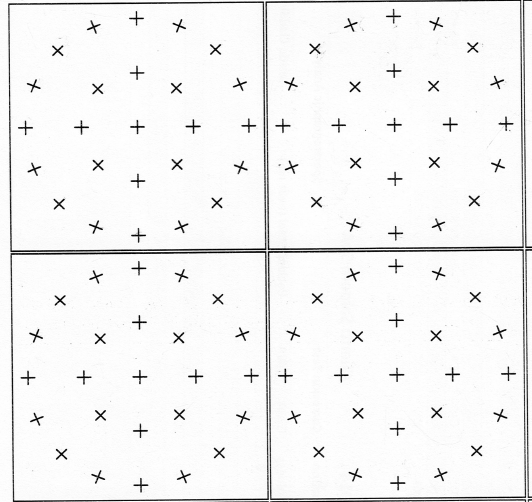
\includegraphics[scale=1]{Bilder/Raster.png}
\caption{Raster für das Auszählverfahren}
\label{Raster für das Auszählverfahren}
\end{figure}

Für eine gleichmäßige Verteilung der Phasen reichen die äußeren Ringe der Felder. Liegen die Anteile allerdings bei wenigen Prozent müssen alle Kreuze berücksichtigt werden. 
Anschließend erfolgt das Auszählen. Die Kreuze die auf der Phase liegen, die bestimmt werden soll, werden mit 1 gezählt. Liegen die Kreuze an einer Phasengrenze, werden sie mit 0,5 gezählt. Berühren die Kreuze die Phase nicht werden sie mit 0 gezählt. Alle Werte werden aufsummiert und durch die Anzahl aller gezählten Kreuze geteilt. Das Ergebnis ist der Phasenanteil. Dieses Verfahren wird an fünf unterschiedlichen Bildbereichen durchgeführt und der Mittelwert gebildet.

\subsection{Zugversuch}

Bei einem Zugversuch werden Proben bis zum Bruch gedehnt und dabei Werkstoffkennwerte bestimmt. Die Kennwerte sind unter anderem  Elastizitätsmodul, Elastizitätsgrenze, Zugfestigkeit und Bruchdehnung. Unter diesen Kennwerten ist für die Anforderung der Arbeit die Zugfestigkeit interessant, da diese über eine Wärmebehandlung optimiert werden soll. Sie ist die größte plastische Dehnung bevor sich das Bauteil einschnürt. Aus diesem Kennwert kann auch die Dauerfestigkeit näherungsweise bestimmt werden, da diese nahezu proportional zur Zugfestigkeit ist. 

\chapter{Wärmebehandlungen}
\section{Festigkeitssteigerung durch Martensitbildung}
Die Literaturrecherchen zeigen, dass sich die mechanischen Eigenschaften der Titanlegierung durch unterschiedliche Gefügestrukturen einstellen lassen. Die erste Methode um die Härte bzw. Zugfestigkeit zu steigern, ist die Einstellung des Primär Alpha Gehalts. Mit einem sinkenden Gehalt der Alpha Phase, steigt die Härte des Gefüges. \cite{Sahoo2015}. Der Alpha Anteil lässt sich mit einer Wärmebehandlung variieren. 
Mit einer Wärmebehandlung im zwei Phasen Gebiet ($\alpha'+ \beta$) sinkt der Anteil der Alpha Phase mit steigender Temperatur, bis die Beta Transustemperatur erreicht ist (siehe Abbildung \ref{Phasendiagram}). Um diesen Anteil beizubehalten muss die Temperatur eine bestimmte Zeit gehalten und anschließend schnell abgekühlt werden. Die Diffusionsvorgänge sollen so klein wie möglich gehalten werden. Neue Alpha Körner sollen nicht entstehen und die vorhandenen Körner sollen nicht auf Kosten der Beta Phase weiter wachsen. Oberhalb der Martensitstarttemperatur kann sich aus der Beta Phase je nach Abkühlmedium Martensit oder transformierte Beta Phase bilden.

\subsection{Abhängigkeit des Primär Alpha Anteils von der Glühtemperatur}
Drei Proben wurden bei jeweils bei 950°C, 960°C und 970°C für eine Stunde im Ofen geglüht und anschließend im Wasser abgeschreckt. Anschließend wurden die Proben präpariert. Die Abbildungen aus \ref{Alle Glühen} zeigen die lichtmikroskopischen Aufnahmen. Primär Alpha Körner liegen in einer Martensit Matrix. Die Alpha Körner wurden durch das Abschrecken eingefroren, und die Beta Phase ist komplett in den Martensit umgeklappt. Die unterschiedlichen Primär Alpha Anteile sind klar zu erkennen.

\begin{figure}
\subfigure[Gefüge bei einer Glühungstemperatur von 970°C]{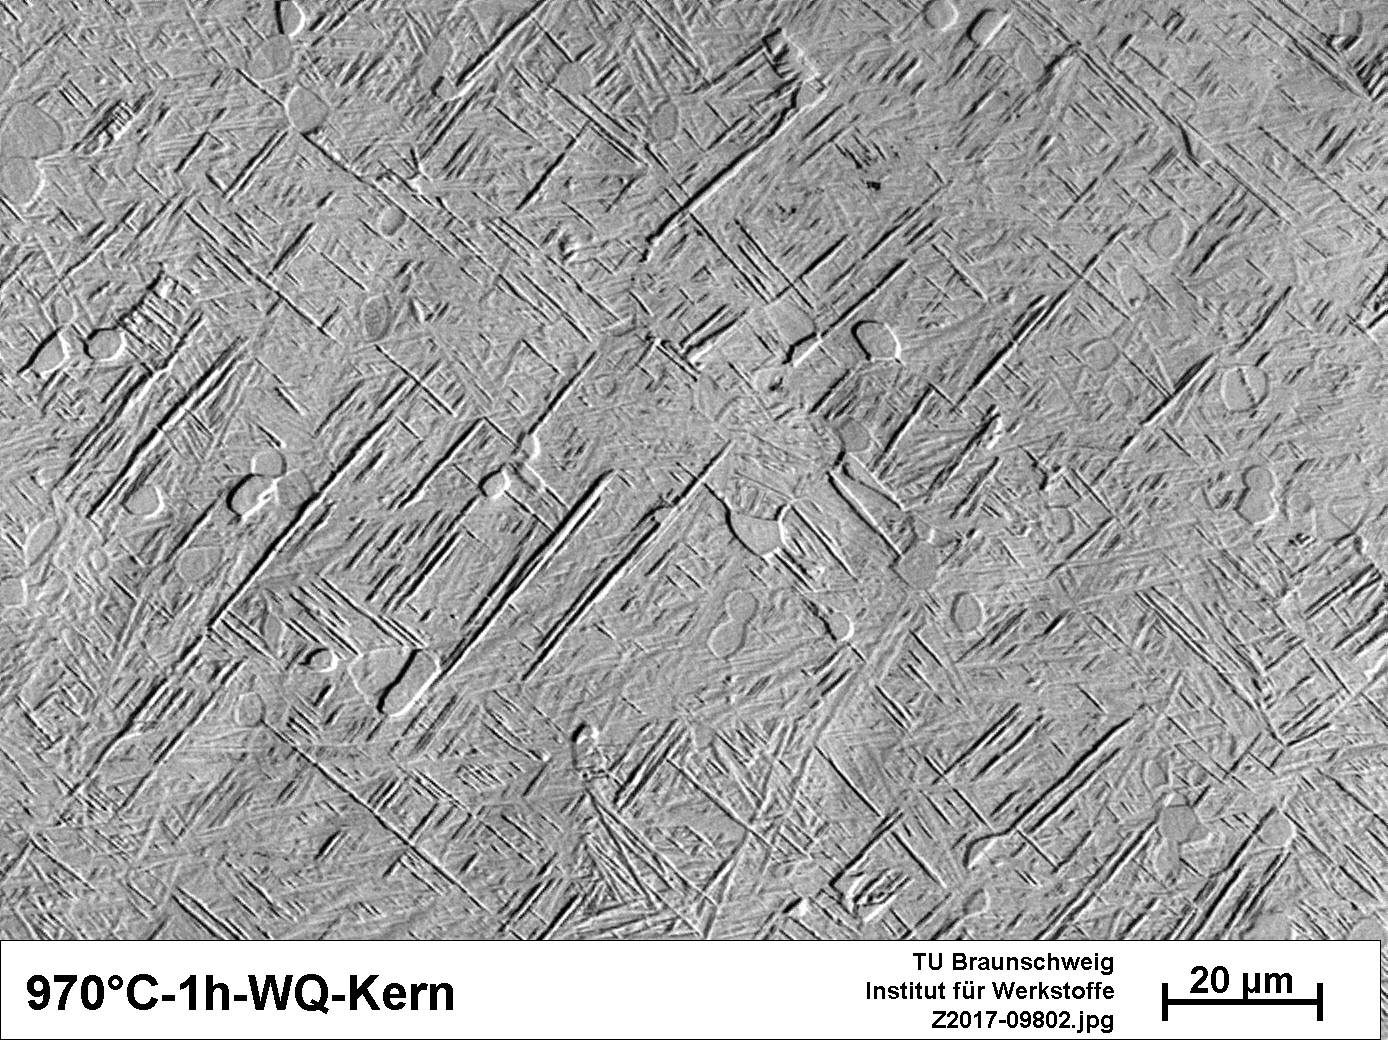
\includegraphics[width=0.33\textwidth]{Bilder/9701hwq.jpg}}
\subfigure[Gefüge bei einer Glühungstemperatur von 960°C]{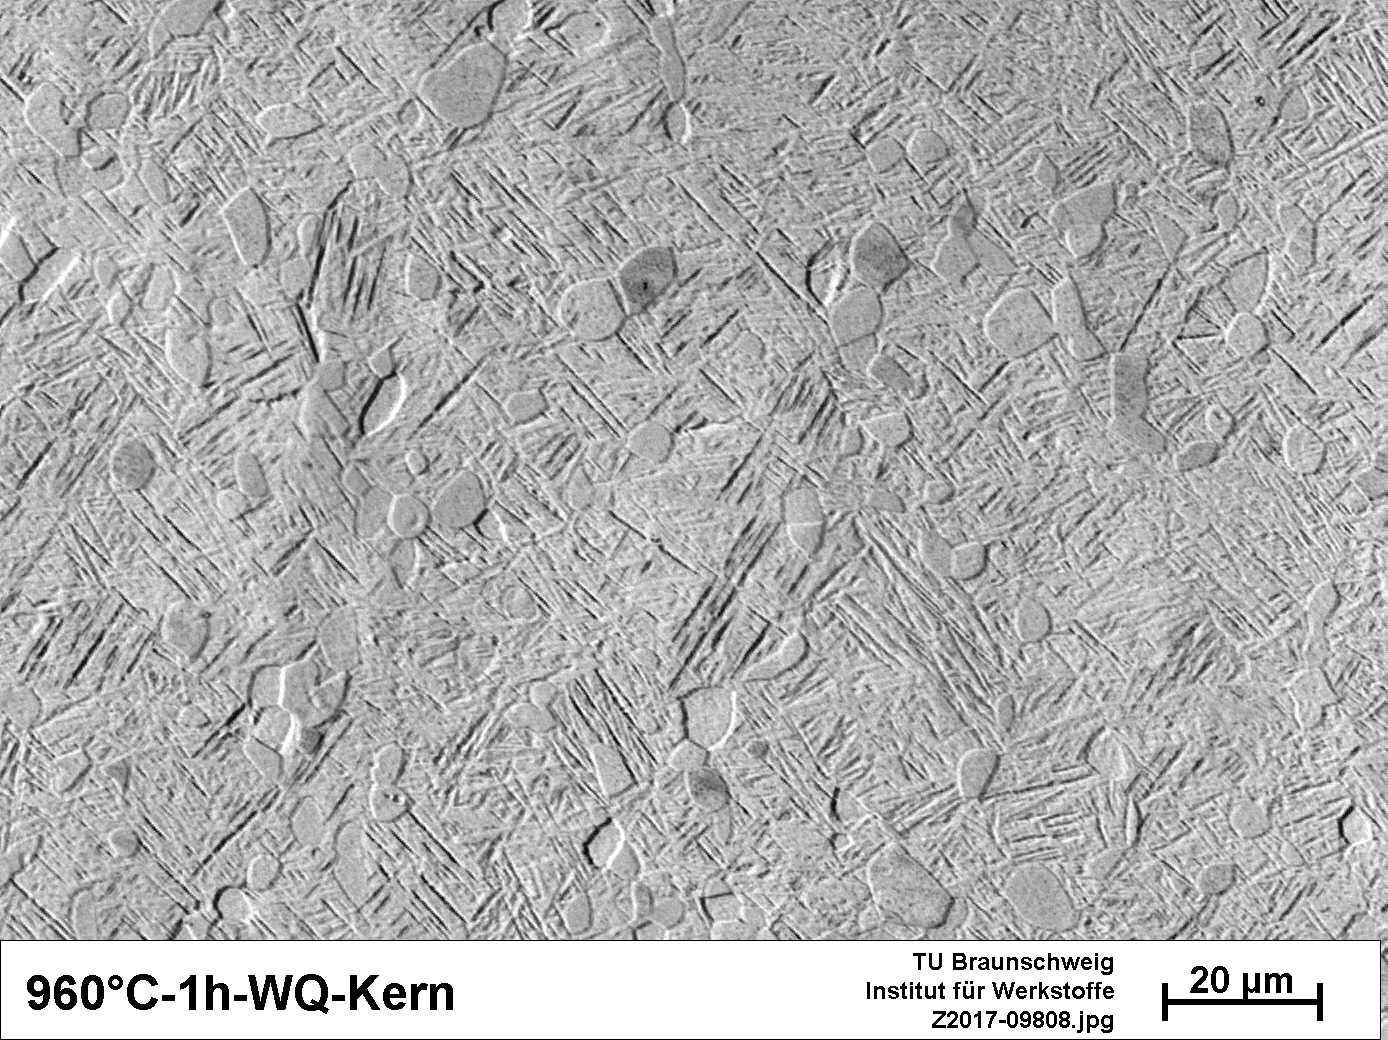
\includegraphics[width=0.33\textwidth]{Bilder/9601hwq.jpg}}
\subfigure[Gefüge bei einer Glühungstemperatur von 950°C]{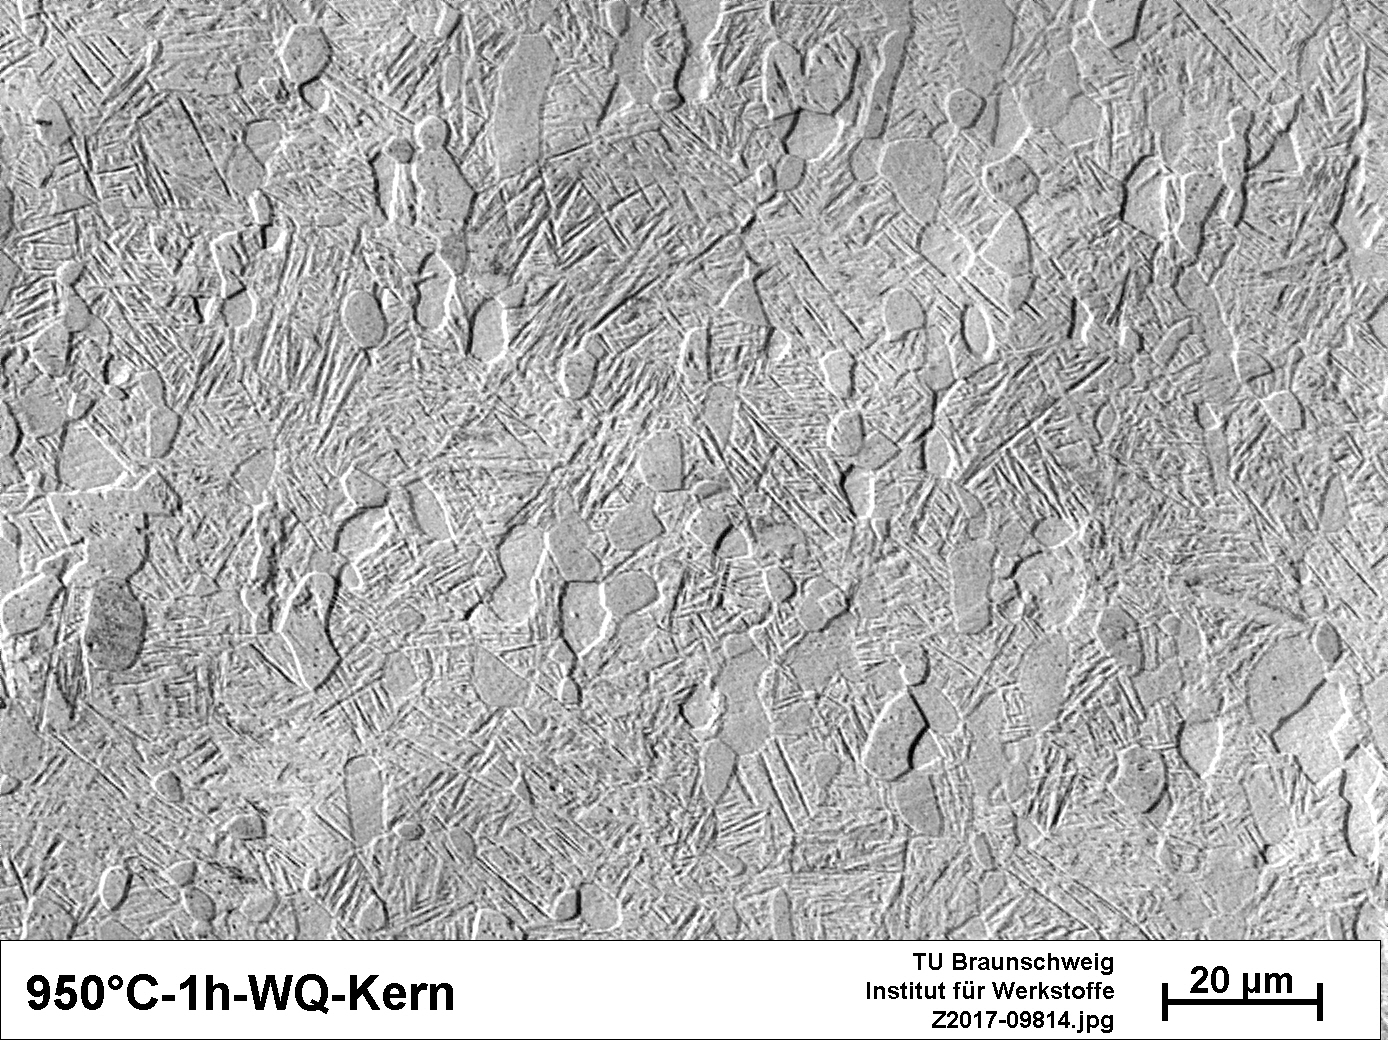
\includegraphics[width=0.33\textwidth]{Bilder/9501hwq.jpg}}
\caption{Gefüge unterschiedlicher Glühtemperaturen}
\label{Alle Glühen}
\end{figure}

Die genauen Phasenanteile wurden mittels Auszählverfahren (2.2.1) bestimmt. Die Ergebnisse zeigt Tabelle \ref{Tabelle Primäralphaanteil}.Bei einer Temperatur von 970°C ist der Alpha Anteil mit  6 \% sehr gering und mittels Lichtmikroskop nur noch schwer zu erkennen. Die 20 \% Alpha bei einer Glühtemperatur von 950°C hingegen sind noch deutlich zu erfassen.
\begin{table}
\begin{tabular}{c | c | c}
Wärmebehandlung & Mittelwert Primäralphaanteil \% & Standardabweichung \\
\hline
950°C 1h WQ	& 20 	&	1,57 \\
960°C 1h WQ	& 13 	&	1,68 \\
970°C 1h WQ	& 6  	&	1,82 \\
\end{tabular}
\caption{Primäralphaanteil in Abhängigkeit der Glühtemperatur}
\label{Tabelle Primäralphaanteil}
\end{table}

\subsection{Abhängigkeit der Härte vom Primäralphaanteil}
Die Härte der Proben wurde mittels der Vickers Härteprüfung bestimmt. Aus fünf Härtemessungen pro Probe wurde ein Mittelwert errechnet. Bei einer Prüfkraft von 10 HV dringt der Prüfkörper in die Alpha Körner und den Martensit ein. Somit entsteht in gemitteltem Härtewert des Gefüges. Die Tabelle \ref{Härte in Abhängigkeit der Glühtemperatur} zeigt eindeutig, dass die Härte mit sinkendem Primär Alpha Anteil steigt. Bei einem Anteil von 20 \% liegt die Härte bei ca. 340 HV10. Sinkt der Anteil auf 6 \%, steigt die Härte auf einen Wert von ca. 360 HV10.

\begin{table}	%Härte in Abhängigkeit der Glühtemperatur
\begin{tabular}{c|c|c|c}
Wärmebehandlung	& Primär Alpha Anteil [\%] &	Mittelwert 
Härte in HV 10 	& Standardabweichung \\
\hline
950°C 1h WQ	& 	20	&	343	&	6,68 \\
960°C 1h WQ	&	13	&	351	&	9,07 \\
970°C 1h WQ	&	6	&	357	&	8,95 \\

\end{tabular}
\caption{Härte in Abhängigkeit der Glühtemperatur}
\label{Härte in Abhängigkeit der Glühtemperatur}
\end{table}
\subsection{Bewertung der Ergebnisse}
Es besteht eine Proportionalität zwischen dem Primär Alpha Anteil und der Härte des Gefüges. Je geringer der Anteil Alpha Phase im Gefüge, desto höher ist die Härte. Der wachsende Anteil des Martensits bewirkt somit die Härtesteigerung. Mit diesem Ergebnis ist zu klären, ob ein vollmartensitisches Gefüge die Härte nochmals steigert. Dieses Gefüge wird im vollgendem behandelt.
Zudem ist die hohe Standardabweichung der Härtewerte auffällig (siehe Anhang Härte Protokolle). Die Härteeindrücke wurden längs durch die Schlifffläche gelegt. Die Härteprotokolle zeigen, dass der erste und der fünfte Messwert oft nach unten ausreißt. Diese Eindrücke liegen nahe der Randzone. Ein Härteabfall in der Randzone könnte mit dem entstandenen $\alpha$-Case \ref{alphacase} zusammen hängen.   

\begin{figure}
\centering
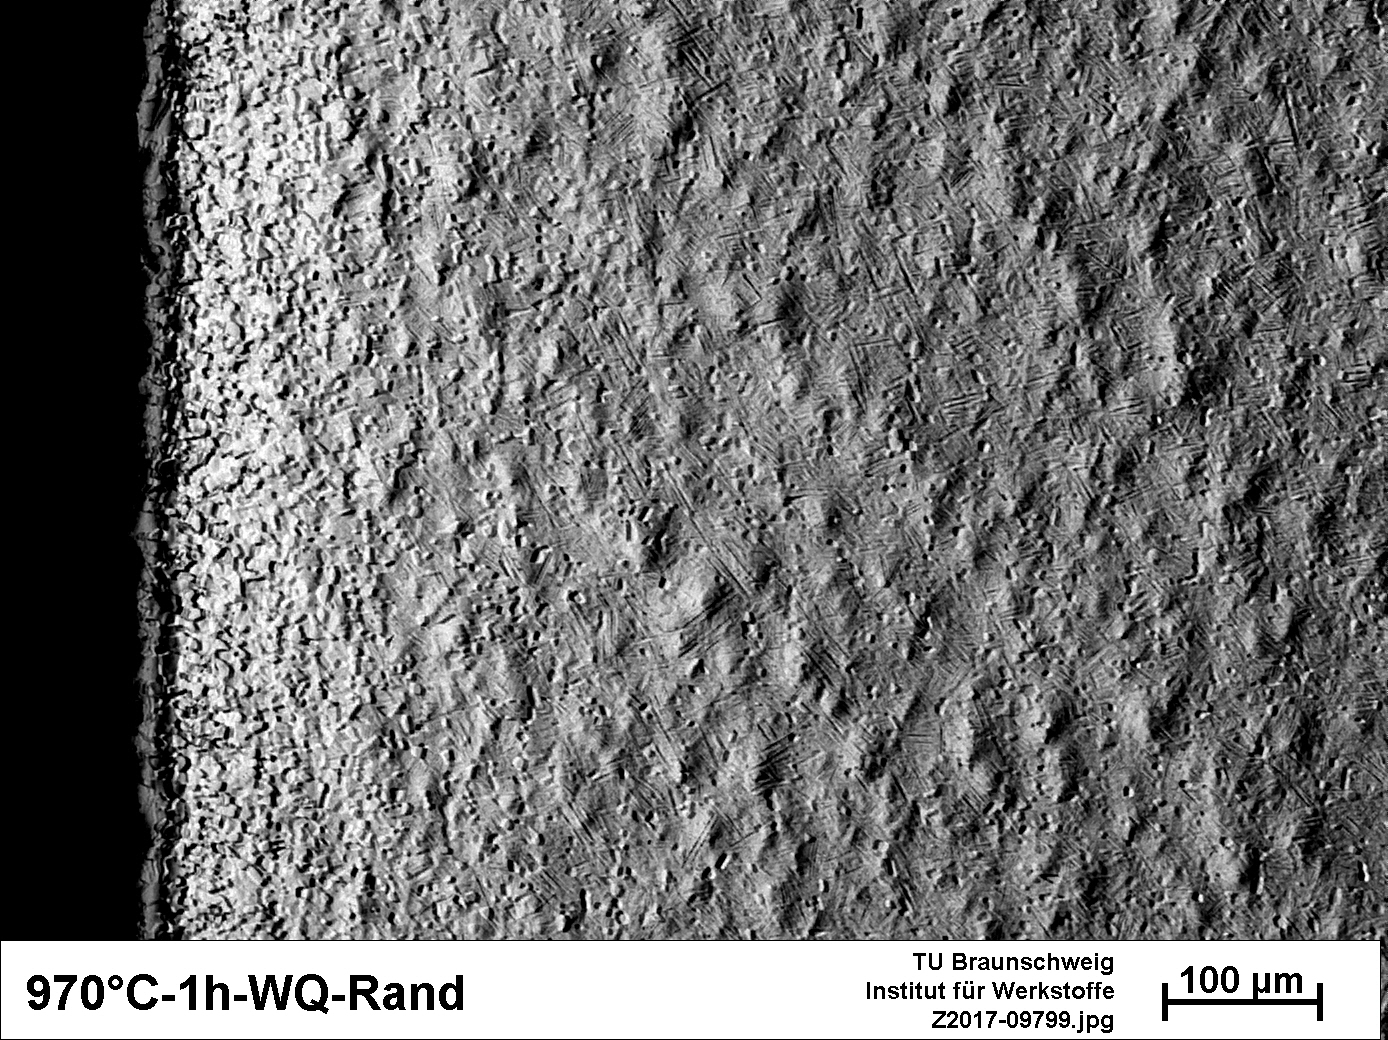
\includegraphics[width=\textwidth]{Bilder/alphacase.jpg}
\caption{Alphacase}
\label{alphacase}
\end{figure}  




\section{Festigkeitssteigerung durch Auslagern des Vollmatensits}
\section{Festigkeitssteigerung durch Auslagern von Primäralpha und Martensit}
In zahlreichen vergleichbaren Untersuchungen wurde bereits eine Festigkeitssteigerung durch Auslagerung von $\alpha + \alpha'$ festgestellt. Auf Basis dieser Untersuchungen und Ergebnissen aus vorherigen Behandlungen werden die Parameter für diese Wärmebehandlung gewählt. 
\subsection{1. Wärmebehandlung}
\cite{Gilbert2004} und \cite{chen2008} geben Beispiele für Erfolgreiche Lösungsglüh- und Alterungsprozesse. Sie dienen als Hilfsmittel für die Parameterwahl bei dieser Strategie zur Festigkeitssteigerung. Bei den Bespielen werden Glühungstemperaturen von 950°C bis 970°C verwendet, sodass ein zweiphasiges Gefüge entsteht. Um $\alpha'$ zu erzeugen wird abgeschreckt. Als Haltezeit wird eine Stunde gewählt. Diese Haltezeit ist ausreichend, damit sich das Gefüge vollständig umwandeln kann.

Wie in Kapitel zwei bereits erläutert sorgen höhere Temperaturen für einen niedrigen Primäralphagehalt. Aus vorherigen Wärmebehandlungen ist für eine hohe Festigkeit, ein möglichst niedriger Primäralphaanteil vorteilhaft. Jedoch ist bei einer anschließenden alternden Behandlung, in der der Martensit optimal zerfallen soll, die Legierungselementanteile in den Phasen wichtig. Bei einem niedrigen Primäralphaanteil ist der Anteil der Alphastabilisierenden Elementen in der Martensitphase größer als bei größeren Primäralphaanteilen, da die Alphaphase nur begrenzt Elemente aufnehmen kann. So verbleiben möglicherweise so große Mengen, dass der Martensit nicht in Alpha und Beta zerfällt und die Alterung ohne Auswirkungen bleibt.

Für die Alterung, mit anschließender Luftkühlung, wurde in den Beispielen eine Temperatur von 490°C bis 595°C und eine Haltezeit von 1 bis 8 Stunden angegeben. Da diese Spanne sehr groß ist und eine aussagekräftige Beurteilung der Ergebnisse für den gesamten Bereich unverhältnismäßig aufwendig sein würde, wurde eine Temperatur festgelegt und über die Haltezeit variiert. So werden in einem ersten Schritt die Auswirkungen des Primäralphaanteils analysiert. Es wurden wasserabgescheckte Proben bei einer Glühungstemperatur von 970°C und 950°C jeweils zwei und acht Stunden bei 520°C gealtert. Es werden also vier Proben verwendet die ein vergleichbares Ergebnis liefern sollen. So kann eine Auswirkung der unterschiedlichen Primäralphaanteile gleichzeitig mit der Auswirkung der Haltedauer beobachtet werden und Rückschlüsse auf die entstehenden Eigenschaften getroffen werden.
\subsection{Ergebnisse 1. Wärmebehandlung}
\subsubsection{970°C Auslagerung}
Auf den Gefügebildern aus Abbildung \ref{970 alterung} kann man unterscheide zu dem Ausgangsgefüge aus Abbildung \ref{Gefüge ohne Alterung}(a) sehen. Die Bereiche des Primäralphas sind unabhängig von der Auslagerungszeit in ihrer Größe konstant geblieben. Dies lässt sich dadurch begründen, dass eine Veränderung des Primäralphagehalts nur bei hohen Temperaturen oder extrem langen Haltezeiten passieren kann. Da beides nicht vorliegt bleibt der Gehalt konstant.

Allerdings kann eine Veränderung des Martensits beobachtet werden. Je länger die Haltezeit desto mehr ist dieser zerfallen. Es bildet sich sekundäres Alpha und Beta, das zufällig dort entsteht wo die jeweiligen stabilisierenden Legierungselemente die größte Konzentration aufweisen. Bei einer Haltezeit von zwei Stunden ist der Zerfall schwer zu erkennen. Die Ausprägung der entstehenden sekundären Alpha- beziehungsweise Betaphase ist sehr gering und die Martensitnadeln sind noch gut zu erkennen. 

Bei einer Haltezeit von acht Stunden ist die Zerfall des Martensits deutlicher zu erkennen als bei der kürzeren Haltezeit. Die Konzentration an Martensitnadeln ist sichtbar geringer und somit ist die Entstehung von Alpha und Beta vorangeschritten. 

Durch eine Härteprüfung lässt sich die Auswirkung der Alterung analysieren. Dabei wird das oben beschriebene Verfahren angewendet. Für die Behandlungsreihe mit 970°C ergeben sich die Ergebnisse aus Tabelle \ref{heartepruefung9702h}. Werden diese Werte mit den Härtewerten des rein abgeschreckten Material aus Tabelle \ref{Hearte ohne Behandlung} verglichen ist eine Erhöhung der Härte zu erkennen. Sie ist durch die Auslagerung um circa 10 HV 10 gestiegen. Für die längere Haltezeit ist der Härtewert konstant. es kann also keine Aussage getroffen werden, ob eine längere Haltezeit mit einer Steigerung der Härte verbunden ist. 

\subsubsection{950°C Auslagerung}
Die Auslagerung bei einer Glühtemperatur von 950°C zeigt ein anderes Ergebnis als die bei einer Glühtemperatur von 970°C. Werden die Gefüge von Abbildung  \ref{Glühung950+alterung} mit dem abgeschreckten Gefüge aus Abbildung \ref{Gefüge ohne Alterung}(b) verglichen erkennt man einen weiter fortgeschrittenen Zerfall des Martensits. Bei einer Alterungszeit von zwei Stunden hat die Menge an Martensitnadeln bereits abgenommen. Bei acht Stunden sind diese kaum noch zu erkennen. Dies spricht dafür, dass die Alterung zu einem stärkeren Zerfall des Gefüges als bei höherer Temperatur geführt hat. 

Bei den Proben die mit 950°C geglüht wurden und zwei beziehungsweise acht Stunden bei 520°C ausgelagert wurden zeigt sich ein ähnliches Ergebnis der Härteprüfung wie bei den Proben auf der höheren Temperatur. Wenn die Härtewerte nach der Alterung mit denen vorher verglichen werden, ist eine Härtesteigerung erkennbar. Die Werte aus der Tabelle \ref{950alterung} sind im Schnitt 10 HV 10 höher als das Material vor der Behandlung. Anders als bei der Behandlung mit den Proben die bei 970°C geglüht wurden bleiben die Härtewerte bei der Auslagerung mit acht Stunden Haltezeit konstant. 
\begin{table}[t]	%Härtewerte ohne Auslagerung
\begin{tabular}{c|c}
\multicolumn{2}{c}{970°C 1h WQ} \\
\hline 
Abstand in mm	& Härte in HV 10 \\
0.03	& 345\\
3.01	& 350\\
6.00	& 343\\
8.98	& 339 \\
11.97	& 342\\
Mittelwert	& 344 \\
Max	& 350 \\
Min.	& 339 \\
Std.-abw. &	4.21 \\

\end{tabular}
\begin{tabular}{c|c}
\multicolumn{2}{c}{950°C 1h WQ} \\
\hline 	
Abstand in mm	& 	Härte in HV 10 \\
-0.01	&	337 \\
3.17	&	347 \\
6.32	&	349 \\
9.48	&	348 \\ 
12.62	&	336 \\
Mittelwert &	343 \\
Max	&	349 \\
Min.	&	336 \\
Std.-abw.	&	6.68 \\

\end{tabular}
\caption{Härtewerte ohne Auslagerung}
\label{Hearte ohne Behandlung}
\end{table}
\begin{table}[t] 	%Härteprüfung 970°C Glühen und Auslagern
\begin{tabular}{c | c}
\multicolumn{2}{c}{2h Auslagern} \\
\cline{1-2}
Abstand in mm & Härte in HV 10 \\
0.03 & 357 \\
3.16 & 358 \\
6.29 & 360 \\
9.43 & 354 \\
12.56 & 359 \\
Mittelwert & 358 \\
Max & 360 \\
Min & 354 \\
Std.-abw. & 2.58 \\
\end{tabular}
\begin{tabular}{c | c}
\multicolumn{2}{c}{8h Auslagern} \\
\cline{1-2}
Abstand in mm & Härte in HV 10 \\
0.07	&		353 \\
2.91	&		352 \\
5.79	&		352\\
8.67	& 		355\\
11.54	& 		357\\
Mittelwert &	354\\
Max	& 			357\\
Min. &			352	\\	
Std.-abw.	&	2.40\\

\end{tabular}
\caption{Härteprüfung 970°C Glühen und Auslagern}
\label{heartepruefung9702h}
\end{table}
\begin{table}[t] 	%950 Alterung
\begin{tabular}{c|c}
\multicolumn{2}{c}{2h Auslagern} \\
\hline
Abstand in mm	& Härte in HV 10 \\
0.01	&	352 \\
2.98	&	356 \\
5.94	&	356 \\
8.90	&	355 \\
11.86	&	358 \\
Mittelwert	&	355 \\
Max	&	358 \\
Min.	&	352 \\
Std.-abw.	&	2.43 \\

\end{tabular}
\begin{tabular}{c|c}
\multicolumn{2}{c}{8h Auslagern} \\
\hline
Abstand in mm	&	Härte in HV 10 \\
0.02	&	357 \\
3.22	&	355 \\
6.42	&	358 \\
9.62	&	357 \\
12.82	&	354 \\
Mittelwert	&	356 \\
Max	&	358 \\
Min.	&	354 \\
Std.-abw.	&	1.83 \\

\end{tabular}
\caption{Härteprüfung 950°C Glühen und Auslagern}
\label{950alterung}
\end{table}
\begin{figure} 		%Gefüge Ohne Alterung
	\subfigure[Gefüge bei einer Glühungstemperatur von 970°C ohne Alterung]{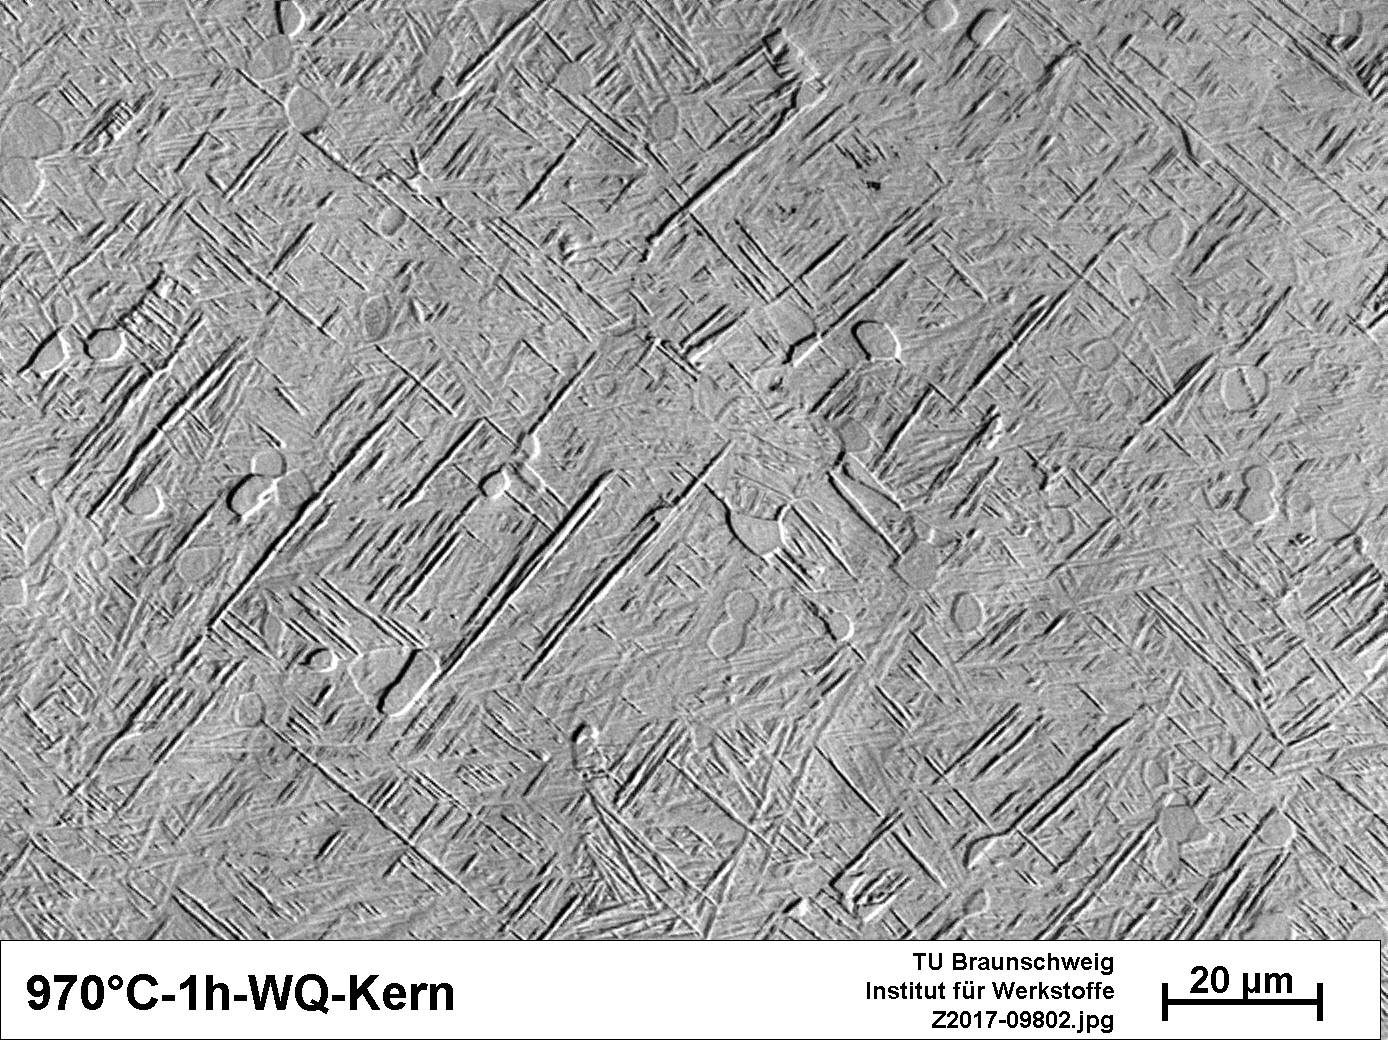
\includegraphics[width=0.49\textwidth]{Bilder/9701hwq.jpg}} 
    \subfigure[Gefüge bei einer Glühungstemperatur von 950°C ohne Alterung]{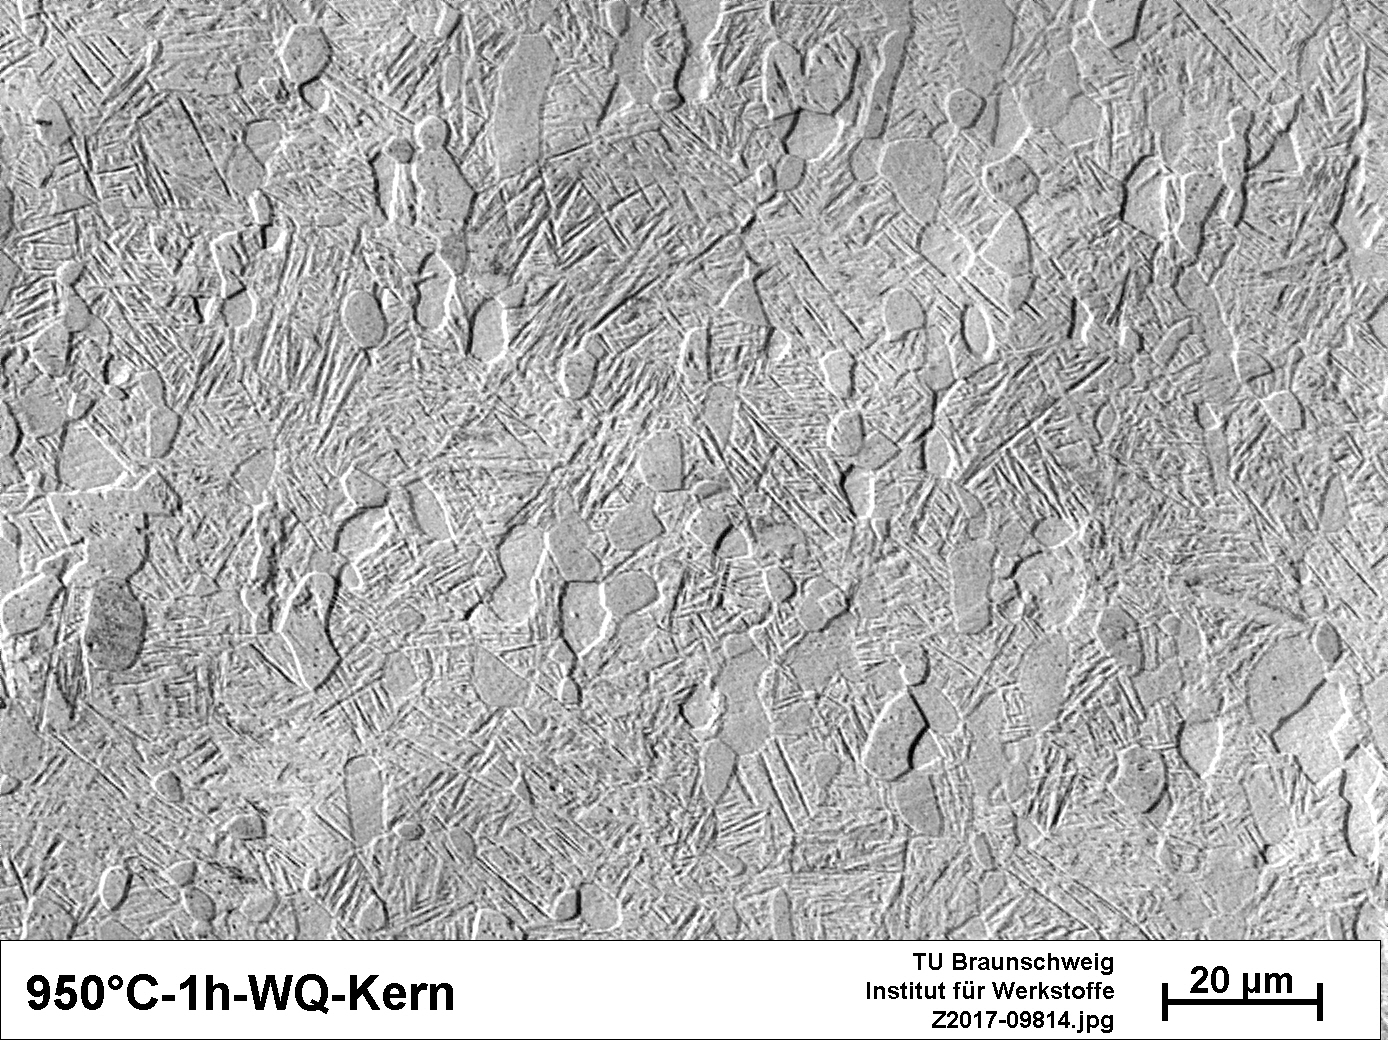
\includegraphics[width=0.49\textwidth]{Bilder/9501hwq.jpg}} 
	\caption{Gefüge ohne Auslagern}
	\label{Gefüge ohne Alterung}
\end{figure}
\begin{figure} 		%970°C und alterung
	\subfigure[Gefüge bei einer Glühungstemperatur von 970°C mit Auslagerung bei 520°C für 2h]{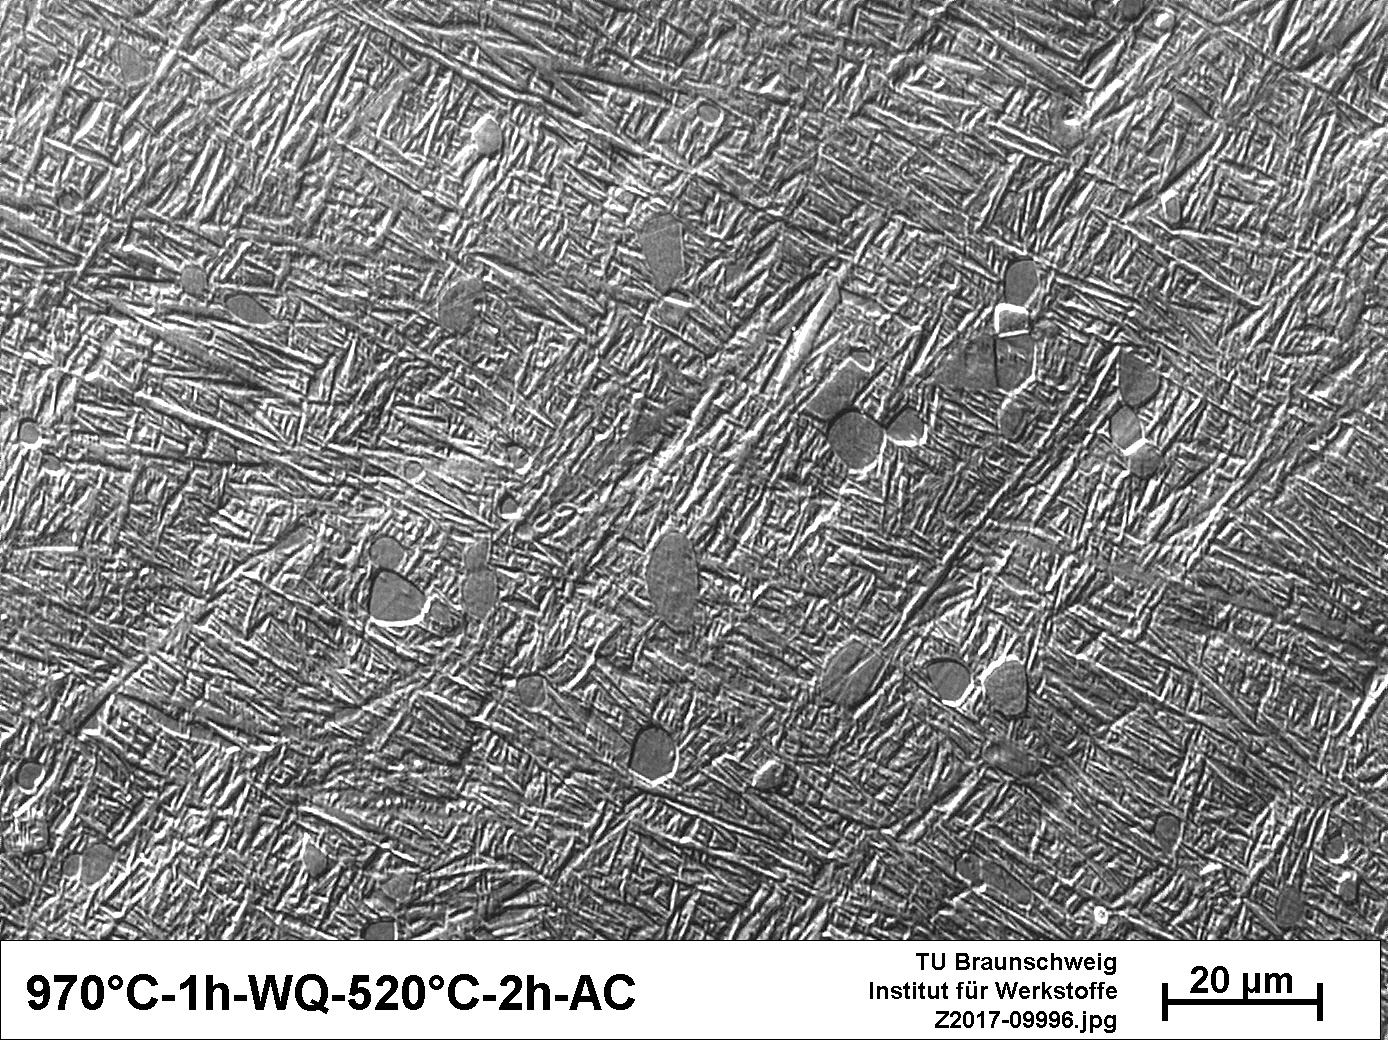
\includegraphics[width=0.49\textwidth]{Bilder/9701hwq5202hac.jpg}} 
    \subfigure[Gefüge bei einer Glühungstemperatur von 970°C mit Auslagerung bei 520°C für 8h]{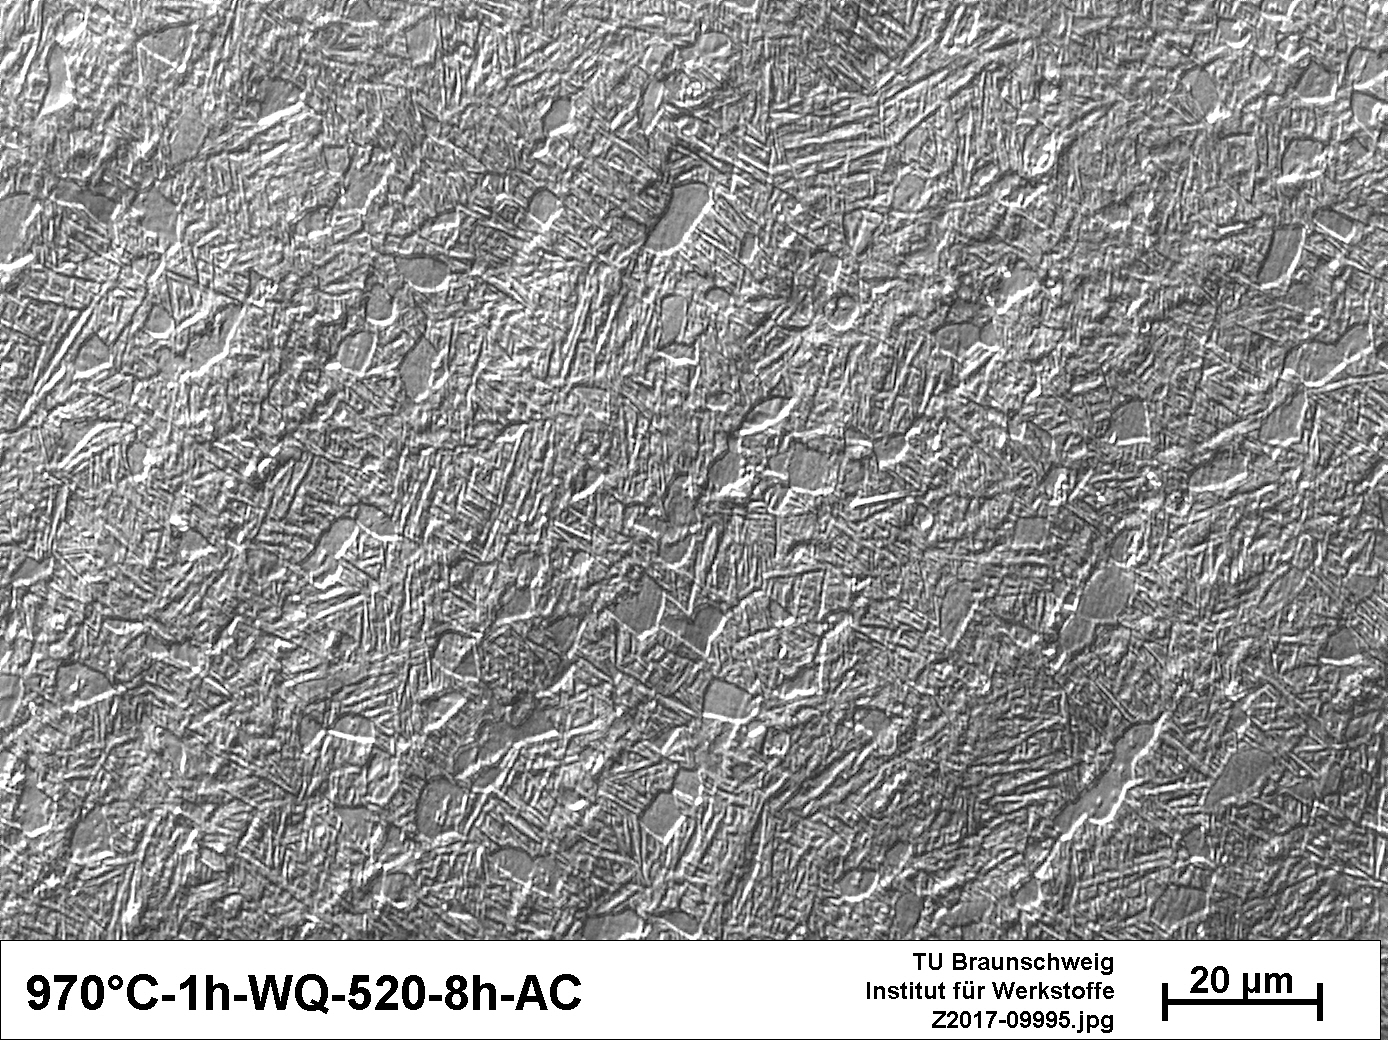
\includegraphics[width=0.49\textwidth]{Bilder/9701hwq5208hac.jpg}} 
    \caption{Gefüge mit einer Glühtemperatur von 970°C und unterschiedlichen Alterungszeiten}
    \label{970 alterung}
\end{figure}



\subsection{2. Wärmebehandlung}
Auf Grund der Ergebnisse der ersten Behandlung ist es denkbar mit der Glühungstemperatur von 950°C weiter zu arbeiten. Es ist wahrscheinlicher, dass der Martensit bei der geringeren Glühungstemperatur besser in Alpha und Beta zerfällt als das Material das eine Glühung bei 970°C widerfahren hat. Die Konzentration an Betastabilisatoren innerhalb des Martensits ist bei einer Glühung von 950°C höher als bei 970°C. Da der Zerfall des Martensits positiv von den Betastabilisatoren abhängt, wird die weitere Behandlung mit einer Glühtemperatur von 950°C durchgeführt.

Die Ergebnisse aus den Härteprüfungen lassen darauf schließen, dass eine Alterung zu einer höheren Härte führt. Daher wird in dem zweiten Schritt die Haltezeit verlängert, um zu Prüfen ob die Härte weiter zu nimmt. Da die Auslagerungstemperatur gering gewählt wurde, könnten die Diffusionsvorgänge in der bisherigen Haltezeit nicht optimal abgeschlossen werden. Die längere Haltezeit würde dazu führen, dass diese weiter fortschreiten könnten. Ob die Härte so gesteigert wird, oder die lange Diffusionszeit dazu führt, dass das Gefüge zu sehr entspannt, wird so erprobt. Nach \cite{Gilbert2004} sind für eine Entspannung des Martensitsgefüge Zeiten von bis zu 50 Stunden realistisch. Diese Zeiten würden aber wahrscheinlich zu einer Abnahme an Härte führen. In folge dessen werden die Zeiten für diesen zweiten Schritt auf 16 und 24 Stunden bei der selben Temperatur festgelegt. So können Langzeitalterungen in ihrer Effektivität eingeschätzt werden. 

\begin{figure} %950°C und alterung
	\subfigure[Gefüge bei einer Glühungstemperatur von 950°C mit Auslagerung bei 520°C für 2h]		{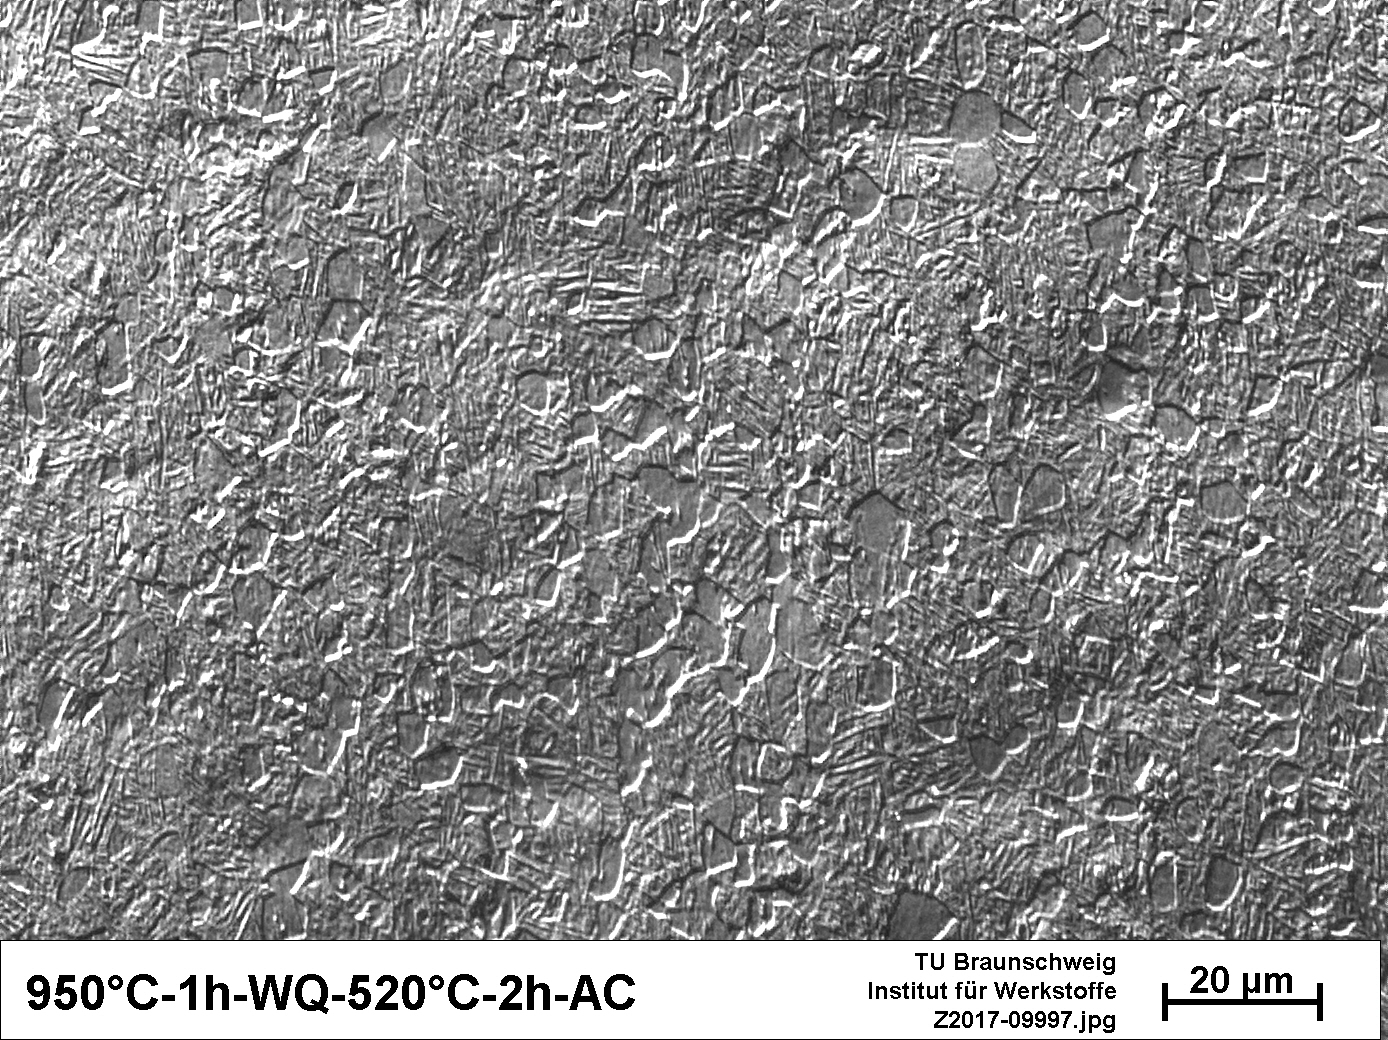
\includegraphics[width=0.49\textwidth]{Bilder/9501hwq5202hac.jpg}} 
    \subfigure[Gefüge bei einer Glühungstemperatur von 950°C mit Auslagerung bei 520°C für 8h]{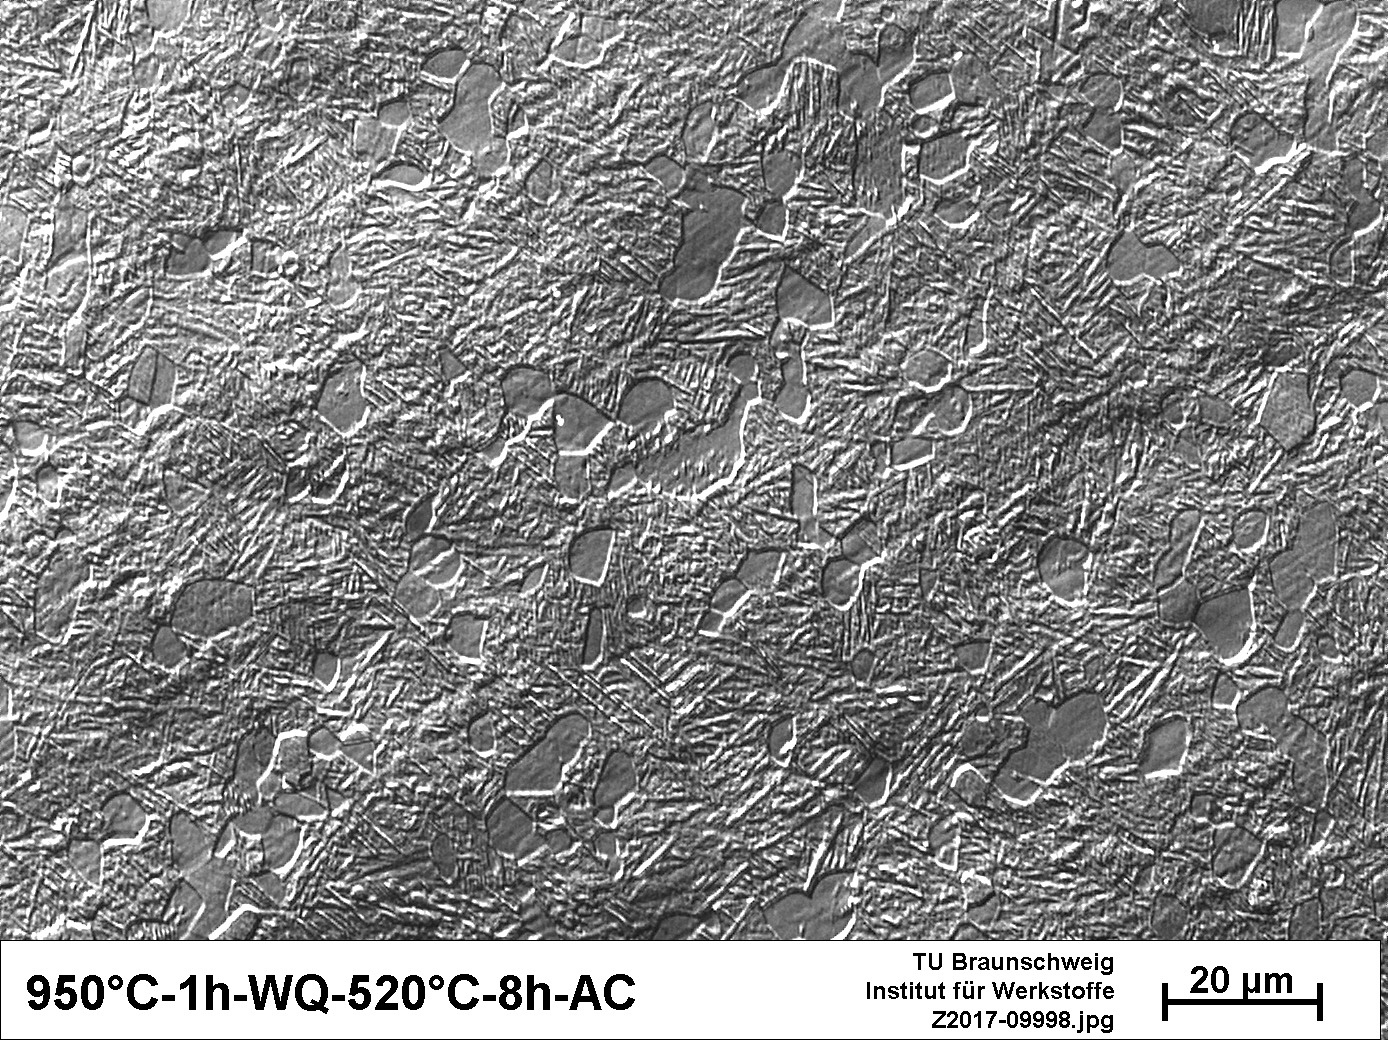
\includegraphics[width=0.49\textwidth]{Bilder/9501hwq5208hac.jpg}} 
    \caption{Gefüge mit einer Glühtemperatur von 950°C und unterschiedlichen Alterungszeiten}
    \label{Glühung950+alterung}
\end{figure}
\subsection{Ergebnisse 2. Wärmebehandlung}
Mit den Gefügebildern aus Abbildung \ref{950 lange auslagerung} wird eine deutlich sichtbarere Ausprägung des Martensitzerfalls festgestellt. Die Bereiche in denen Sekundäralpha und Beta entstanden ist, sind nun deutlicher zu erkennen. Bei der Alterung mit 16 Stunden Haltezeit zeigt sich ein Unterschied hinsichtlich der Dicke der entstandenen Nadeln zu der mit einer Haltezeit von 8 Stunden. Die längere Haltezeit sorgt für eine größere Ausprägung dieser Nadeln. Bei einer Haltezeit von 24 Stunden ist dieser Effekt noch deutlicher zu beobachten. Die Nadeln heben sich nun von einander ab und bilden lamellenartige Strukturen. Das Martensit kann nur noch schwierig zwischen den entstandenen Lamellen erkannt werden. Es spricht somit dafür, dass der Zerfall sehr weit fortgeschritten ist. 



\begin{figure}
\subfigure[Gefüge bei einer Glühungstemperatur von 950°C und 16 Stunden Alterung]{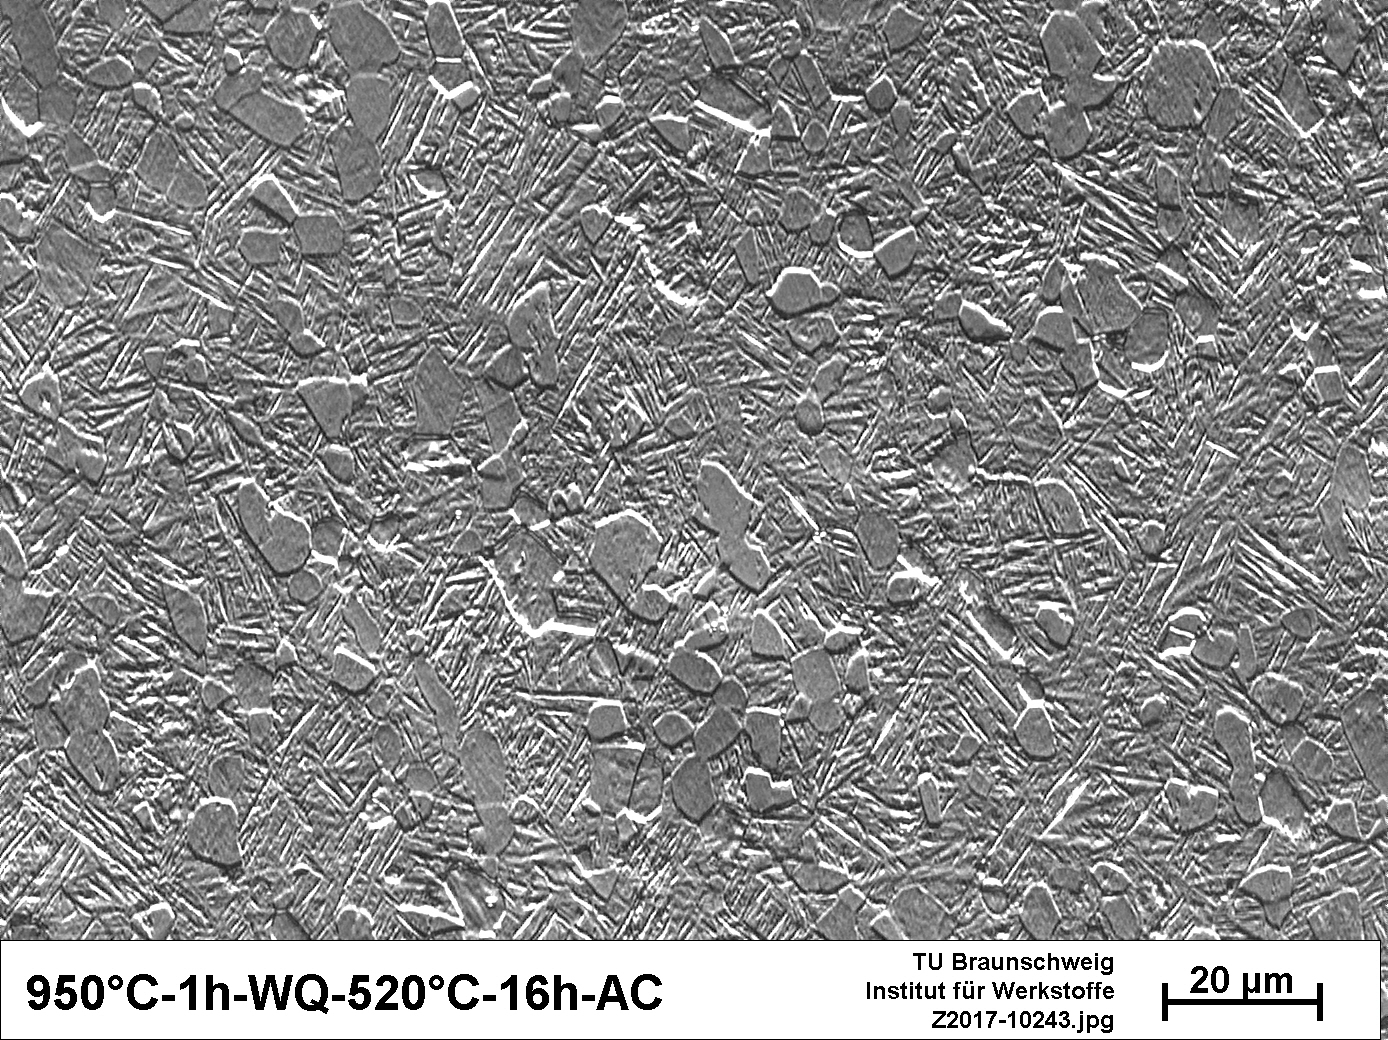
\includegraphics[width=0.49\textwidth]{Bilder/9501hwq52016hac.jpg}} 
    \subfigure[Gefüge bei einer Glühungstemperatur von 950°C und 24 Stunden Alterung]{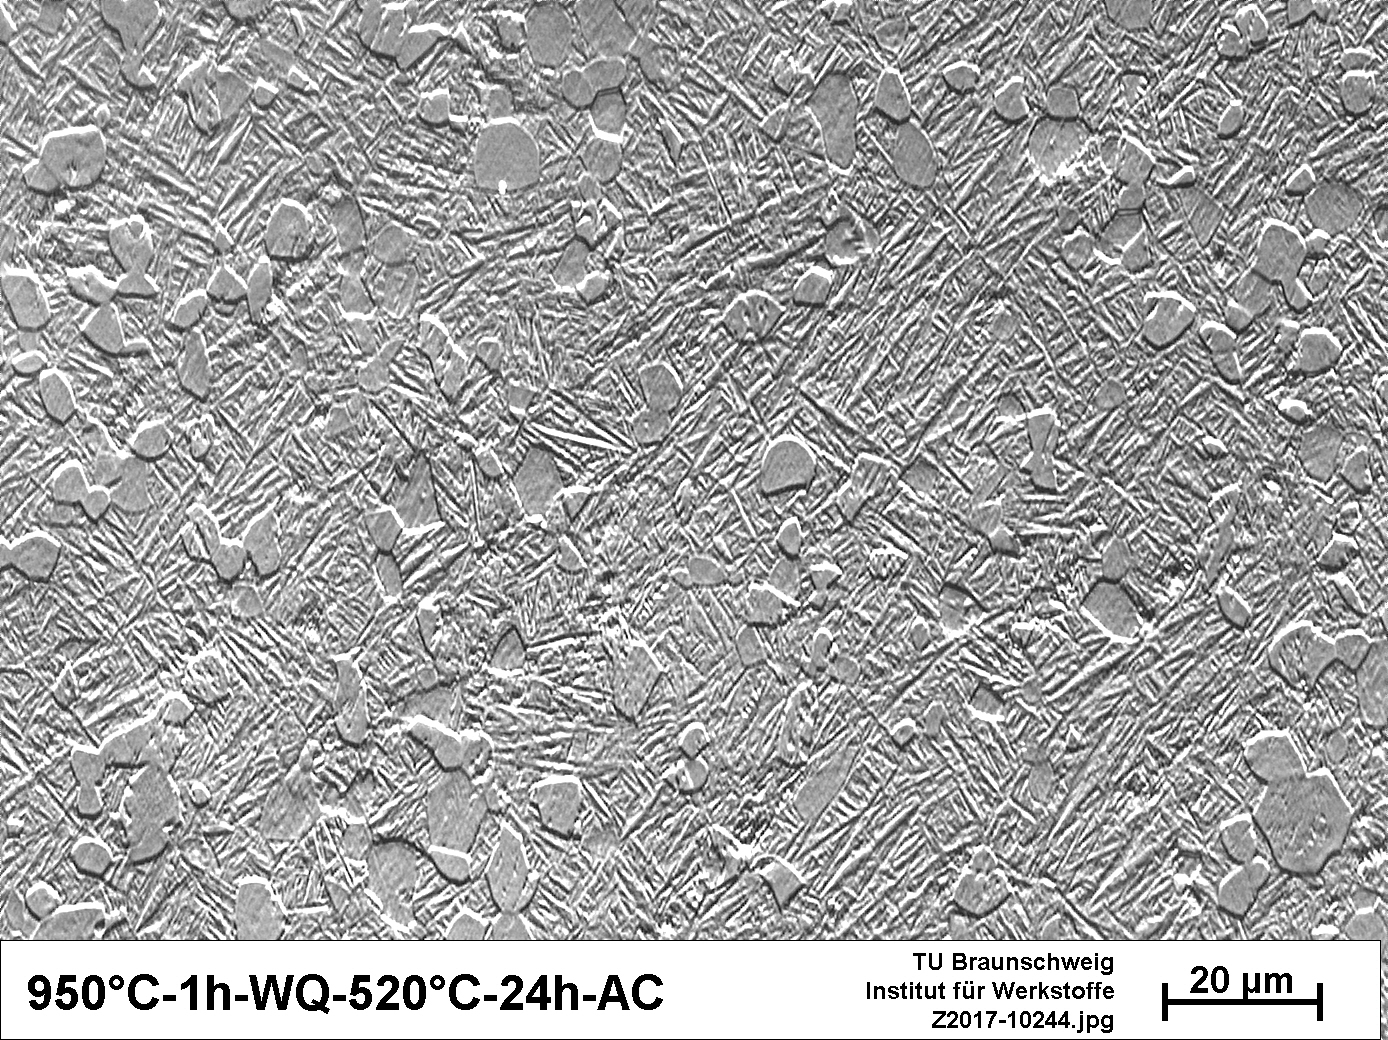
\includegraphics[width=0.49\textwidth]{Bilder/9501hwq52024hac.jpg}} 
	\caption{Gefüge bei 950°C bei 16h und 24h Auslagerung}
	\label{950 lange auslagerung}
\end{figure}
\bibliographystyle{plain}
\bibliography{literatur}
\listoffigures
\listoftables
\end{document}
